\documentclass[12pt,letterpaper,oneside,openright]{report}
%\usepackage{geometry} 
\RequirePackage{amsmath}
\usepackage[spanish]{babel}
\usepackage[latin1]{inputenc} %help babel
%\usepackage{listings}

%Agregando el fancy stuff
\usepackage{fancyhdr} % Necesario para los encabezados
\usepackage{fancyvrb}
\usepackage{makeidx} % En caso de necesitar indices.


\usepackage{amssymb}
\usepackage{epstopdf}
\usepackage{longtable}
\usepackage{color}
\usepackage{indentfirst}
\usepackage{algorithm}
\usepackage{algorithmic}
% Traducir algorithm
\floatname{algorithm}{Algoritmo}

\usepackage[table]{xcolor}
\usepackage{caption}

% to include pdf cover page
\usepackage{pdfpages}

\numberwithin{algorithm}{section}
\newcommand{\theHalgorithm}{\arabic{algorithm}}

\usepackage{hyperref}
\hypersetup{
  pdfborder={0,0,0}
}

%Happy chapters
\usepackage{sectsty}
\chapterfont{\Large\centering\thispagestyle{empty}}

%Margins:
\usepackage[left=3cm,right=2cm,top=2.5cm,bottom=2cm]{geometry}
\setlength{\headheight}{15pt}

%% Commented to accept double sided 

%\hoffset=-0.41in %1.5cm left margin: 1in - 0.41in
%\marginparwidth = 2.5cm %3.0cm margin notes as left margin
%\oddsidemargin = 1.6cm
%\marginparsep = 0.1cm
%\textwidth = 16.5cm %to make right margin 2cm and not margin notes
%\voffset=-0.22in %2cm upper margin: 1in - 0.22in
%\topmargin = 0.5cm %after upper margin before chapter 2cm+topmargin(3cm)
%\headheight = 12pt
%\footskip = 0.5cm
%\headsep = 25pt
%\textheight = 21.11cm %

%Equation numeration
\usepackage{amsmath}
%\numberwithin{equation}{subsection}
\numberwithin{equation}{section}

%Linespacing 1.5
\usepackage{setspace}
\onehalfspacing  


%Graphic manipulation
\usepackage{graphicx}
\graphicspath{{./images/}} %images path
\usepackage{float}

%For figure wrapping
\usepackage{wrapfig}

%For subfloats
\usepackage{subfig}

%enumeration depth
%\setcounter{secnumdepth}{3}

%compile just these 'include' tags
%\includeonly{chapter1,chapter2,chapter3,chapter4,chapter5} 
\includeonly{abstract-spa,chapter1-spa,chapter2-spa,chapter3-spa,chapter4-spa,chapter5-spa}

%\title{Algoritmo de detecci\'on de gusanos en im\'agenes de microscopio}
\title{Procesamiento de im\'agenes para detectar \\
gusanos C. elegans}
\author{Javier Fern\'andez}

\begin{document}
\renewcommand{\tablename}{Tabla}
\renewcommand{\listtablename}{\'Indice de tablas}
\renewcommand{\chaptername}{CAP\'ITULO}

%Rename Algorithmic commands
\floatname{algorithm}{Algoritmo}
\renewcommand{\listalgorithmname}{Lista de algoritmos}
\renewcommand{\algorithmicrequire}{\textbf{Entrada:}}
\renewcommand{\algorithmicensure}{\textbf{Salida:}}

%\setlength{\parskip}{0pt}
%\maketitle

%\includepdf[pages=1]{cover/cover}
%\thispagestyle{empty}
%\cleardoublepage
%\includepdf[pages=1]{cover/abstract}
%\thispagestyle{empty}
%\cleardoublepage

% Pagina de titulo
% Pagina de titulo
\begin{titlepage}
\begin{center}

% Upper part (aqui ya esta incluido el logo de la USB).
\includegraphics[scale=0.5,type=png,ext=.png,read=.png]{images/cebolla} \\

% Encabezado
\textsc {\large UNIVERSIDAD SIM\'ON BOL\'IVAR} \\
\textsc{\bfseries DECANATO DE ESTUDIOS PROFESIONALES\\
COORDINACI\'ON DE INGENIER\'IA DE LA COMPUTACI\'ON}

\bigskip
\bigskip
\bigskip
\bigskip
\bigskip
\bigskip
\bigskip
\bigskip
\bigskip

% Title/Titulo
% Aqui ponga el nombre de su proyecto de grado/pasantia larga
\textsc{\bfseries PROCESAMIENTO DE IM\'AGENES PARA DETECTAR \\
GUSANOS C. ELEGANS}

\bigskip
\bigskip
\bigskip
\bigskip
\bigskip

% Author and supervisor/Autor y tutor
\begin{minipage}{\textwidth}
\centering
Por: \\
JAVIER FERN\'ANDEZ \\

\bigskip
\bigskip
\bigskip

Realizado con la asesor\'ia de: \\
ALEXANDRA LA CRUZ\\
JOHAN HENRIKSSON
\end{minipage}

\bigskip
\bigskip
\bigskip
\bigskip
\bigskip
\bigskip
\bigskip
\bigskip
\bigskip

% Bottom half
{PROYECTO DE GRADO \\ Presentado ante la Ilustre Universidad Sim\'on Bol\'ivar \\
como requisito parcial para optar al t\'itulo de \\ Ingeniero en Computaci\'on} \\

\bigskip
\bigskip
\vfill

% Date/Fecha 
{\large \bfseries Sartenejas, Diciembre de 2010}

\end{center}
\end{titlepage}


\setcounter{secnumdepth}{3}
\setcounter{tocdepth}{4}


% Define encabezado numeros romanos y como se separan los captiulos y las
% secciones
\addtolength{\headheight}{15pt}
\pagenumbering{roman}
\pagestyle{fancyplain}

\renewcommand{\chaptermark}[1]{\markboth{\chaptername\ \thechapter:\,\ #1}{}}
\renewcommand{\sectionmark}[1]{\markright{\thesection\,\ #1}}


\lhead{}
\chead{}
\rhead{}
\renewcommand{\headrulewidth}{0.5pt}
\lfoot{}
\cfoot{\fancyplain{}{\thepage}}
\rfoot{}

\begin{abstract}

   % What is C. elegans and why is it so important.
   % The problem: manual assays are to intensive, need
   % for automated solutions.
   % What do we provide: a image processing methodology that
   % provides semi-automatic solution, for Endrov (open source
   % image analysis software)
   % Few methods attempt to resolve cluttering. Individual
   % images are not usually addressed (large datasets).
   % Automated solutions fit 85 percent of the image. We 
   % fit 100% 

El nematodo C. elegans es un organismo ampliamente
utilizado. Posee muchas c\'elulas con equivalentes humanos y otras
condiciones especialmente favorables, que lo han convertido en modelo
de estudio para la biolog\'ia, especialmente la gen\'etica del
desarrollo. As\'i mismo, al ser peque\~no y transparente se presta bien
a una gran variedad de t\'ecnicas de cribado de alto rendimiento
(HTS). \\ 

La identificaci\'on de gusanos deber\'ia automatizarse lo m\'as
posible dado que es muy trabajoso efectuarla manualmente.
En este trabajo se presenta un algoritmo de procesamiento de im\'agenes
para detectar C. elegans en im\'agenes obtenidas por microscop\'ia de 
alto rendimiento. As\'i mismo, se provee una metodolog\'ia general 
de detecci\'on de gusanos. La soluci\'on semi-autom\'atica que aqu\'i se presenta, 
permite identificar eficazmente gusanos individuales en agrupaciones de gusanos. En
t\'erminos generales, el proceso  consta de lo siguiente:
una imagen dada es segmentada, separando as\'i grupos de gusanos del
fondo de la imagen. Se detectan gusanos individuales de manera autom\'atica, siguiendo un
proceso de comparaci\'on y ajuste de siluetas de gusanos. Este proceso
se basa en encontrar siluetas factibles dentro de una agrupaci\'on, 
minimizando la distancia que existe entre dicha agrupaci\'on y 
siluetas gen\'ericas que son deformadas para ajustarse a ella.
Las conformaciones de gusanos ajustadas incorrectamente 
pueden ser corregidas f\'acilmente de manera manual.\\

La soluci\'on provista presenta un enfoque innovador para
detectar exitosamente gusanos C. elegans individuales en 
im\'agenes de microscopio. Los resultados muestran que esta soluci\'on
semi-autom\'atica permite detectar, correctamente, la forma del 100\% de 
los gusanos presentes en una imagen determinada.
Por lo general, el proceso es completado en menos de minuto y medio
para im\'agenes con alta densidad de gusanos. 
En im\'agenes con baja densidad, los gusanos
pueden ser identificados en su totalidad de manera enteramente 
autom\'atica. La precisi\'on de la detecci\'on y el tiempo requerido 
para calcularla son mejorados notablemente con respecto a la
identificaci\'on manual.\\

La soluci\'on fue implementada en \emph{Java} e integrada a
\emph{Endrov}, una arquitectura de extensiones de c\'odigo abierto para
an\'alisis de im\'agenes, y esta siendo utilizada en el Departamento de
  Biociencias y Nutrici\'on del Instituto Karolinksa, Flemingsberg, Suecia.

\end{abstract}

\tableofcontents
\listoftables
\listoffigures

\fancyhf{} % Redefine el encabezado 
\lhead{}
\chead{}
\rhead{\fancyplain{}{\thepage}}
\renewcommand{\headrulewidth}{0.5pt}
\lfoot{}
\cfoot{}
\rfoot{}


%must be below \tableofcontents: paragraph indentation
\setlength{\parindent}{10pt} %look for 3-spaces in late
%\cleardoublepage
\thispagestyle{empty}
\chapter{INTRODUCCI\'ON}
\pagenumbering{arabic}

\section{Motivaci\'on y Prop\'osito}
\label{sec:motivation}

El nematodo C. elegans es un organismo ampliamente utilizado
y se ha convertido en un importante modelo de estudio para la
biolog�a, especialmente la gen�tica del desarrollo.
Este organismo presenta la ventaja de que todos los individuos son exactamente
iguales a nivel celular, poseen cortos ciclos de vidas y una r�pida
gen�tica. Por esta raz�n, se pueden detectar tipos salvajes de este organismo 
y los experimentos son menos costosos, en comparaci�n 
con organismos m�s complejos. Es el �nico animal del que se conoce
cada divisi�n celular, desde la fertilizaci�n del huevo hasta la etapa
adulta, as� como el diagrama completo de las conexiones de esas
c�lulas.\\

El C. elegans tiene muchas c�lulas con equivalentes humanos, lo que 
hace posible estudiar y comprender como se manifiestan ciertas
enfermedades y condiciones relacionadas, e.g. adicci�n a las drogas,
envejecimiento, disfunci�n de ciertas prote�nas, etc.
As� mismo, al ser peque�o y transparente, se presta bien
a una gran variedad de t�cnicas de cribado de alto rendimiento
(HTS). El HTS es un m�todo de experimentaci�n cient�fica que permite
conducir millones de pruebas gen�ticas, bioqu�micas o farmacol�gicas,
a trav\'es de la rob\'otica, software de control y procesamiento de datos,
dispositivos para el manejo de l\'iquidos y detectores sensitivos.
A trav�s de este proceso se pueden identificar r�pidamente componentes
activos, anticuerpos o genes que modelan procesos biomoleculares
particulares, tal como se indica en \cite{highthroughput}. \\
Diversos ganadores del premio Nobel de Medicina o Fisiolog�a
han centrado sus estudios en gusanos, y en particular C. elegans, 
tales como Brenner, Sulston y Horvitz (2002), Fire y Mello (2008),
as� como el ganador del Nobel de Qu�mica, Martin Chalfie (2008).\\

Antes de ser cuantificados, los gusanos deben ser identificados. Este
proceso deber�a ser autom�tico debido a que es muy trabajoso para
ser efectuado manualmente en un tiempo factible. Curiosamente, a 
pesar de la utilidad del C. elegans para manipulaciones gen�ticas,
su utilizaci�n en procesos de cribado de alto rendimiento se
ha visto tambi\'en limitado por la necesidad de ensayos manuales 
muy trabajosos.\\

Esto conlleva a la necesidad de m\'etodos m\'as r\'apidos y consistentes.
Por esta raz\'on, un programa de computadora que permita detectar individuos 
C. elegans en im\'agenes digitales, proveer\'ia una soluci\'on autom\'atica
para el problema de reconocimiento. Esto mejorar\'ia tanto la precisi\'on como 
el tiempo requerido para la identificaci\'on de los individuos, con respecto
a la identificaci\'on manual, permitiendo, a su vez, transformar 
las im\'agenes en informaci\'on manejable.\\

El presente estudio, se centra en el dise\~no e implementaci\'on de un 
algoritmo de procesamiento de im\'agenes para detectar 
gusanos C. elegans en im\'agenes de microscopio. Se provee,
as\'i mismo, una metodolog\'ia general de detecci\'on de gusanos.
La caracter\'istica m\'as relevante para la 
mayor\'ia de los experimentos con C. elegans es la forma del 
gusano, y en ocasiones tambi\'en la rotaci\'on y direcci\'on de la misma.
El enfoque que aqu\'i se presenta, busca identificar, exclusivamente, 
la forma de los gusanos. Se estudia, entonces, si es posible detectar 
y ajustar estas formas de manera automatizada, y si esto puede
alcanzarse m\'as r\'apidamente que a trav\'es de la identificaci\'on manual.\\

Se utilizan gusanos, en estado de larva, en placas de microtitulaci\'on. Las
larvas se cultivan en medio l\'iquido, lo que causa que el fondo de las im\'agenes
sea muy claro. No obstante, los gusanos se solapan con frecuencia.
La implementaci\'on es integrada a \emph{Endrov}, una arquitectura de extensiones
de c\'odigo abierto, dirigida al an\'alisis de im\'agenes y procesamiento de datos,
que fue desarrollada y es actualmente utilizada en el
Departamento de Biociencias y Nutrici\'on del Instituto Karolinksa, lugar donde
se desarrolla este proyecto.


\begin{itemize}
\item Objetivo General
  \begin{itemize}
  \item Dise\~nar e implementar una metodolog\'ia basada en procesamiento de
    im\'agenes para detectar gusanos en im\'agenes de microscopio.
  \end{itemize}
\end{itemize}
\begin{itemize}
\item Objetivos Espec\'ificos
  \begin{itemize}
  \item Dise\~nar un algoritmo de detecci\'on de gusanos que reciba como 
entrada im\'agenes de gusanos en cultivo l\'iquido y retorne la forma 
de los gusanos presentes.
    \begin{itemize}
    \item Revisar los antecedentes relevantes en t\'ecnicas de segmentaci\'on de im\'agenes
    \item Dise\~nar un descriptor de forma y un m\'etodo de rasterizaci\'on para representar gusanos en t\'erminos num\'ericos.
    \item Revisar los antecedentes en ajuste de formas y reconocimiento
      de objetos, y proponer un enfoque de detecci\'on.
    \end{itemize}
  \item Implementar el algoritmo de detecci\'on dise\~nado, integr\'andolo 
    a \emph{Endrov} como extensi\'on.
  \end{itemize}
\end{itemize}


\section{Antecedentes}

La utilizaci\'on del C. elegans en experimentos que involucran 
cribado gen\'etico y qu\'imico se ha incrementado r\'apida y notablemente. 
Esto ha dado pie al desarrollo de
m\'etodos automatizados para analizar su comportamiento, en experimentos 
conducidos sobre grupos de estos organismos, tal como se indica en \cite{automated}.
En el estudio mencionado, se dividen las estrategias existentes para an\'alisis automatizado 
del C. elegans en tres grandes grupos, de acuerdo a su
enfoque metodol\'ogico. Estos son: seguimiento del comportamiento general,
detecci\'on y medici\'on de comportamientos distintos, y medici\'on completa
del comportamiento utilizando grandes conjuntos de datos. Todas estas
estrategias incluyen una etapa fundamental, que se centra
en la detecci\'on de los gusanos en el conjunto de im\'agenes que se utilizan.
El enfoque de detecci\'on var\'ia de una estrategia a otra, pero, por lo general,
comprende los procesos siguientes: extracci\'on de los gusanos del fondo de la imagen (segmentaci\'on), 
\emph{skeletonization} de las formas extra\'idas y parametrizaci\'on 
del contorno de los gusanos.\\ 

La \emph{skeletonization} y subsecuente parametrizaci\'on, se han convertido en un 
m\'etodo est\'andar. Sin embargo, dado que las propiedades de la imagen tales como
iluminaci\'on, ruido y desorden (e.g. huevos y rastros de gusanos) pueden variar
fuertemente de una imagen a otra y debido a que la segmentaci\'on depende directamente del
contexto visual, los par\'ametros de este \'ultimo proceso resultan altamente variables.
Los m\'etodos de segmentaci\'on m\'as utilizados en im\'agenes de gusanos comprenden:
cerrado morfol\'ogico, llenado de agujeros, m\'etodo del valor umbral y sus 
combinaciones.\\

La parametrizaci\'on de gusanos, que consiste en la descripci\'on de formas de gusanos
en t\'erminos num\'ericos, determina la variedad de formas que pueden ser
obtenidas a trav\'es de la asignaci\'on de diferentes valores a los par\'ametros.
El enfoque m\'as com\'un se centra en definir par\'ametros que permitan
la reproducci\'on de una forma de gusano gen\'erica, normalizada para la 
posici\'on, orientaci\'on y escala de un esqueleto de gusano.\\

En \cite{automated}, se sostiene que entre aquellos programas que 
hacen seguimiento de m\'ultiples gusanos, muy pocos intentan resolver
el problema de solapamiento, que surge cuando dos o m\'as gusanos
se cruzan entre s\'i, o bien cuando gusanos individuales se enrollan,
lo que suele llevar a detecciones incorrectas o faltantes. 
Pese a que hay algoritmos que est\'an siendo desarrollados para resolver
este problema, tal como se indica en \cite{huang}, se sigue careciendo
de soluciones que permitan detectar la totalidad de los individuos
de forma autom\'atica.\\

Estudios muy recientes presentan nuevos enfoques para detectar gusanos 
individuales en agrupaciones enredadas (aquellos donde ocurre solapamiento).
Riklin Raviv et al. \cite{individual1} presentan un enfoque para extraer
objetos enredados, basado en sus propiedades morfol\'ogicas. Este estudio
aborda el problema de desenredar agrupaciones de C. elegans en experimentos
de cribado de alto rendimiento. Este m\'etodo se basa en conceptos de 
aprendizaje de m\'aquina y teor\'ia de grafos, y utiliza el esqueleto 
del gusano como descriptor de forma. Los segmentos de agrupaciones de gusanos
son representados como v\'ertices de grafo y se lleva a cabo una b\'usqueda
de los caminos de gusanos m\'as prometedores en el grafo. La detecci\'on
de los descriptores de forma m\'as prometedores dentro de la b\'usqueda
es guiada por una distribuci\'on de probabilidad, basada en el modelo
probabil\'istico presentado en \cite{individual2}.\\ 
Los enfoques presentados en \cite{individual1,individual2} corresponden
a estudios consecutivos y complementarios centrados en la detecci\'on de
gusanos individuales en im\'agenes digitales.
 Los resultados presentados indican un porcentaje de detecci\'on acertada 
de 89\% del total de la muestra, en promedio.
Es importante destacar que los dos estudios previamente mencionados fueron
desarrollados al mismo tiempo que el presente trabajo y con similares
fechas de finalizaci\'on, por lo que hab\'ia desconocimiento de su existencia. 
No obstante, el enfoque de detecci\'on y la metodolog\'ia presentada en este
trabajo, dista bastante de los estudios mencionados.\\


Existen entonces, diversos estudios en procesamiento de im\'agenes
y visi\'on artificial que tratan el an\'alisis automatizado del 
C. elegans y de nematodos en general. La mayor\'ia de estos 
estudios se centran en la locomoci\'on de gusanos, donde el proceso
de identificaci\'on y seguimiento es realizado a trav\'es del procesamiento
simult\'aneo de un conjunto de im\'agenes y no solo una. 
Se evidencian tres procesos fundamentales en las estrategias de 
detecci\'on como lo son: segmentaci\'on de la imagen, esqueletonizaci\'on y 
parametrizaci\'on de forma. El resto de los procesos involucrados en la
detecci\'on var\'ian dependiendo del enfoque, e involucran, en casi todos los casos,
el procesamiento de conjuntos de im\'agenes y no de im\'agenes individuales, 
como fue antes mencionado.\\

A pesar de que algunos m\'etodos automatizados de detecci\'on de gusanos
son capaces de detectar correctamente una gran parte de la muestra, pocos intentan
resolver el problema del solapamiento de gusanos y ninguno lo
soluciona exitosamente.


\section{Estructura del documento}
El presente documento est\'a divido de la siguiente forma:
\begin{itemize}
\item \textbf{Cap\'itulo 1: Introducci\'on}\\
  Se desarrolla la motivaci\'on y el prop\'osito de este estudio. Luego, se
  presentan los antecedentes en detecci\'on de gusanos, indicando los 
  diferentes enfoques, logros y dificultades persistentes.
\item \textbf{Cap\'itulo 2: Marco Te\'orico}\\
  Se abarca la teor\'ia relacionada con el problema y la soluci\'on
  planteada, destacando por t\'opico, los diferentes enfoques que han sido
  previamente estudiados.
\item \textbf{Cap\'itulo 3: Metodolog\'ia de la Soluci\'on}\\
  Se presenta la metodolog\'ia general de la soluci\'on.
  Primero, se desarrolla el razonamiento que sustenta la soluci\'on propuesta.
  Seguidamente, se explica cada etapa de la metodolog\'ia, justificando el enfoque
  escogido. Por etapa, se presentan los detalles de implementaci\'on 
  m\'as relevantes, que dan origen al algoritmo desarrollado en este trabajo.
\item \textbf{Cap\'itulo 4: Experimentos y Resultados}\\
  Se presentan los experimentos llevados a cabo para evaluar el rendimiento
  de la soluci\'on propuesta. El prop\'osito y caracter\'isticas de cada
  experimento son descritos. Luego, se presentan y discuten los resultados
  obtenidos.
\item \textbf{Cap\'itulo 5: Conclusiones y Observaciones Futuras}\\
  Las conclusiones del trabajo son presentadas, as\'i como algunas
  observaciones futuras.
\end{itemize}

%avoid page number on blank pages when cleared
\thispagestyle{empty}
\cleardoublepage
\chapter{Marco Te\'orico}
\label{sec:dev}
\section{Endrov}
\label{sec:endrov}

\emph{Endrov}, es una arquitectura de extensiones de c\'odigo abierto,
dirigida al an\'alisis de im\'agenes y procesamiento de datos.
Se encuentra implementada en \emph{Java}, es portable, y puede ser ejecutada localmente o como 
un \emph{applet}, como se indica en \cite{web:endrov}. \emph{Endrov} surgi\'o
de la necesidad de un software avanzado de c\'odigo abierto que permitiese procesar 
los complejos datos espacio-temporales presentes en im\'agenes de microscopios, 
utilizadas en la investigaci\'on biol\'ogica.\\

\emph{Endrov}, tiene como objetivo mejorar las funcionalidades del software c\'odigo abierto
de an\'alisis de im\'agenes \emph{ImageJ}, proveyendo un dise\~no mas moderno. 
Las deficiencias principales de \emph{ImageJ} son: falta de soporte de metadatos,
no existe soporte real de 5D, la arquitectura de extensiones es confusa, las vistas
no pueden ser extendidas fácilmente, y el procesamiento de lotes es complicado, 
tal como se indica en \cite{web:endrovhome}.
Otros problemas que inspiraron la creaci\'on de \emph{Endrov} fueron: la ausencia de un 
formato de im\'agen estandarizado, y la dificultad
de almacenar datos complejos en los formatos abiertos que existen actualmente.
El grupo de desarrollo cre\'o el formato OST para manejar grandes conjuntos de im\'agenes.
Puede almacenar todo tipo de informaci\'on, pero se encuentra optimizado para im\'agenes.\\

\emph{Endrov}, es tanto una liber\'ia como un programa de an\'alisis y procesamiento de 
im\'agenes. El dise\~no se realiz\'o haciendo fuerte enf\'asis en separar el c\'odigo
de la interfaz gr\'afica de los tipos de datos, filtros y otras extensiones para 
procesamiento de datos. La idea del programa es proveer una herramienta robusta para
an\'alisis y procesamiento de im\'agenes que pueda cubrir las necesidades de aquellos
laboratorios, grupos de investigacion y cualesquiera otros tipos de usuario, que 
manipulan im\'agenes diariamente, \cite{web:endrov}.\\

\emph{Endrov} fue desarrollado por el \emph{TBU Group} del Instituto Karolinska en Suecia, y 
fue liberado oficialmetnte el 17 de Junio de 2009, bajo la licensia BSD.


\section{M\'etodo del Valor Umbral}
\label{sec:thresholding}

Los m\'etodos del valor umbral (MVU), mejor conocidos por su nombre en ingles: \emph{thresholding},
son un conjunto de algoritmos para segmentar gr\'aficos rasterizados, que permiten separar
objetos presentes en una im\'agen del resto. Esta segmentaci\'on es usualmente representada
a trav\'es de una im\'agen binaria, que se obtiene despu\'es de procesar la im\'agen original 
en escala de grises.\\

Una imagen binaria es un tipo de imagen discreta, en la cual cada pixel tiene asignado uno de
dos valores posibles (tipicamente $1$ o $0$). Cada valor indica si el pixel
pertenece al primer o segundo plano (fondo) de la im\'agen original, respectivamente.
Como se indica en \cite{web:thresholding}, durante la ejecuci\'on de un m\'etodo del valor
umbral, se marcan pixeles individuales como p\'ixeles objeto o pixeles de fondo, seg\'un
corresponda. Asumiendo que los objetos en las im\'agenes son mas brillantes que el fondo,
un pixel se marca como pixel objeto si su valor de luminosidad (u otro valor unidimensional) 
es mayor que un valor umbral determinado, de otro modo se marca como pixel de fondo.
Esta conveci\'on se denomina \emph{umbral por encima}. Diferentes variantes incluyen:
\emph{umbral por debajo}, que es el opuesto al anterior; \emph{umbral por dentro}, donde un
pixel es marcado como objeto si su valor de comparaci\'on se encuentra entre dos 
umbrales; y \emph{umbral por fuera}, que es el opuesto a \emph{umbral por dentro}, seg\'un
se explica en \cite{shapiro}.\\


En las aplicaciones de procesamiento de im\'agenes donde el estudio se enfoca en 
objetos particulares contenidos en una imagen, los MVU se convierten en una herramienta
sencilla para separar estos objetos del fondo, aunque no siempre precisa. En \cite[p.146]{thres},
se mencionan diversas aplicaciones en procesamiento de im\'agenes que involucran MVU, tales
como: an\'alisis de im\'agenes de documentos, donde el objetivo es extraer caracteres, logos,
contenido gr\'afico o notas musicales entre otros; procesamiento de mapas, que se centra en
encontrar l\'ineas, leyendas y caracteres; procesamiento de escenas, donde se busca detectar
un objetivo o blanco; e inspecci\'on de calidad de materiales, donde se desea delinear piezas
defectuosas, entre muchos otros.\\

El par\'ametro clave para los MVU es el valor umbral (o valores umbrales para los enfoques de
\emph{umbral por dentro} y \emph{umbral por fuera}). El valor puede ser tanto calculado
automaticamente, como establecido o ajustado manualmente. Los diferentes MVU pueden ser categorizados 
de acuerdo de la informaci\'on que explotan. En \cite[p.147]{thres}, Sezgin y Sankur
categorizan los MVU en seis gr\'upos principales: m\'etodos basados en histograma de formas,  
m\'etodos basados en agrupamiento, m\'etodos basados en entrop\'ia, m\'etodos espaciales y
m\'etodos locales.\\

En la Figura \ref{fig:thres1}, se muestran dos im\'agenes: una en escala de grises y la 
otra, la imagen binaria obtenida a trav\'es de un m\'etodo del valor umbral.

\begin{figure}[h t b p ! H]
  \centering
  \subfloat[Imagen en escala de grises]{\label{fig:threso}\includegraphics[width=0.45\textwidth]{thres/winter_o}}
\qquad
  \subfloat[Imagen binaria obtenida a trav\'es de un m\'etodo del valor umbral]{\label{fig:thres1}\includegraphics[width=0.45\textwidth]{thres/winter_thres}}
  \caption[Im\'agen en escala de grises antes y desp\'ues de aplicar un m\'etodo del valor umbral ]{Im\'agen en escala de grises antes y desp\'ues de 
    aplicar un m\'etodo del valor umbral. Las im\'agenes fueron tomadas de \cite{web:thresholding}}
  \label{fig:thres1}
\end{figure}

\section{Transformada de Distancia}
\label{sec:dt}

Una transformada de distancia o mapa de distancias es una representaci\'on de
una imagen digital, en la cual a cada pixel de la im\'agen le corresponde
un valor que indica la distancia entre ese pixel y el pixel mas cercano que pertenezca
al fondo de la imagen. Se calcula a partir de una im\'agen binaria, que consista
en pixeles de objeto y pixeles de fondo. La imagen que se obtiene corresponde a
una especie de representaci\'on en escala de grises del primer plano de la im\'agen
binaria (conformado por los objetos).\\
El valor mapeado para cada pixel, depende directamente de la funci\'on de distancia,
que define el patron de medici\'on de distancia entre pixeles de la imagen. Existen
diversas funciones de distancia tales como: \emph{Manhattan},
\emph{tablero de ajedrez}, \emph{Euclideana}, \emph{Chamfer 3-4} y \emph{Octogonal}, 
\cite[p.363]{dtresearch}. As\'i mismo, existen muchas otras funciones de
distancia, normalmente derivadas de las anteriormente mencionadas.
En la Figura \ref{fig:dtexamples}, se muestra el resultado de aplicar 
diferentes funciones de distancia a una imagen que contiene un punto en el centro,
rodeado por un fondo blanco.

\begin{figure}[h t b p ! H]
 \centering
   \includegraphics[scale=0.4]{dt/dtref}
 \caption[Distancias a partir de un punto para seis transformadas de distancia]{ 
   Distancias a partir de un punto para seis transformadas de distancia. Mientras 
   mas claro es el color, mas larga es la distancia \cite[p.365]{dtresearch}}
 \label{fig:dtexamples}
\end{figure}

Como se indica en \cite{dtresearch2}, las transformadas de distancia juegan un rol
central en la comparaci\'on de im\'agenes binarias, particularmente aquellas
resultantes de t\'ecnicas de detecci\'on de caracter\'isticas locales, tales 
como detecci\'on de contornos o detecci\'on de esquinas.
Las transformadas de distancia pueden ser interpretadas, tambi\'en, como
topograf\'ias de islas, donde la etiqueta o valor de cada pixel indica la altura o 
profundidad de la regi\'on. De esta forma, se pueden detectar crestas y picos, 
que constituyen la base principal de met\'odos sencillos para encontrar el 
esqueleto topol\'ogico de objetos en im\'agenes, tal como se explica en \cite[237]{ridgedt}.
Las transformadas de distancias son tambi\'en herramientas muy \'utiles para el 
mejoramiento de la eficiencia de algoritmos de morfolog\'ia, tales como: 
\emph{reducci\'on de contornos} and \emph{expansi\'on de contornos}.\\

\section{Esqueletizaci\'on}
\label{sec:skeletonization}

Un esqueleto topol\'ogico es una representaci\'on compacta y simple de un objeto, que
consiste en una versi\'on reducida o delgada del mismo, que es equidistante a sus bordes, 
y que preserva muchas de las caracter\'isticas topologicas y geom\'etricas de la
imagen original, tal como se explica en \cite{wikipedia:skeleton,ssm,augmented}. 
Por lo general, el esqueleto se define como el conjunto de los centros de los discos m\'aximos
contenidos en la imagen original, \cite{ssm,augmented}. Existen muchas otras definiciones diferentes,
que dependen, principalmente, de la forma en que el esqueleto es generado.
Independientemente de la definici\'on que se adopte, si los puntos pertenecientes al esqueleto
son calculados en relaci\'on con su distancia a los bordes originales del objeto, 
el esqueleto puede ser utilizado para reconstruir con exactitud la figura original.
La figura \ref{fig:genskeleton} presenta el esqueleto de una silueta de caballo, y la
imagen binaria a partir de la cual fue calculado el esqueleto.

\begin{figure}[h t b p ! H]
  \centering
  \subfloat[Imagen Binaria]{\includegraphics[scale=0.8]{skeleton/horsebinary}}
\qquad
  \subfloat[Esqueleto topol\'ogico]{\includegraphics[scale=0.8]{skeleton/horseskeleton}}
  \caption[Imagen binaria de una figura de caballo y su esqueleto]{Imagen binaria de una figura de
caballo y su esqueleto. Im\'agenes tomadas de \cite{ssm}}
  \label{fig:genskeleton}
\end{figure}


Los esqueletos topol\'ogicos pueden ser categorizados en diferentes tipos.
Telea et al, \cite{augmented}, describen tres tipos de esqueleto de acuerdo a la forma en que
son calculados, tales como: \emph{esqueleto por reducci\'on morfol\'ogica}, 
\emph{esqueleto por m\'etodos geom\'etricos} y \emph{esqueleto por transformada de distancia}.
El m\'etodo de \emph{reducci\'on morfol\'ogica} consiste en la reducci\'on iterativa de los bordes
del objeto, identificando y marcando, capa por capa, aquellos puntos cuya remoci\'on no afecte
la topolog\'ia del objeto. Estos m\'etodos son sencillos, por lo general, aunque suelen requerir
heur\'isticas complejas para asegurar la conectividad del esqueleto, como se indica en
\cite{augmented}. En \cite{onepass} y \cite{thinning}, se describen dos enfoques paralelos
eficientes para garantizar la conectividad de esqueletos producidos a trav\'es 
\emph{reducci\'on morfol\'ogica}.\\
Los \emph{m\'etodos geom\'etricos} se centran en calcular el diagrama de Voronoi de una
representaci\'on pol\'igonal de los bordes del objeto. El diagrama de Voronoi representa
el eje medio de los bordes. Tal como se asegura en \cite[p.251]{augmented}, estos m\'etodos
producen un esqueleto conectado y preciso, pero son muy complejos de implementar, requieren
una robusta discretizaci\'on de los bordes, y son computacionalmente costosos.\\
El tercer tipo comprende los m\'etodos que calculan el esqueleto a partir de 
la transformada de distancia. El enfoque com\'un consiste en encontrar los puntos cresta
y conectarlos, \cite{maxima, euclideancentre, ridgedt}. Por lo general, estos m\'etodos
pueden garantizar que los puntos esqueletos encontrados son precisos y acertados, 
pero no la conectividad del esqueleto, ni su completitud.\\

El esqueleto topol\'ogico es una herramienta importante para la representaci\'on
y reconocimiento de objetos, en diferentes areas, tales como: visi\'on artificial,
an\'alisis de im\'agenes, y procesamiento de im\'agenes digitales, incluyendo 
reconocimiento \'optico de caracteres, reconocimiento de huellas digitales, inspecci\'on
visual, reconocimiento de patrones, compresi\'on de im\'agenes binarias y plegamiento
de proteinas, \cite{skprotein}.


\section{Ajuste de Formas}
\label{sec:shapefitting}

El ajuste de formas (en ingl\'es \emph{shape matching}), es un problema
central en los sistemas de informaci\'on visual, visi\'on artificial, 
reconocimiento de patrones y rob\'otica, \cite{matchingbook}. Consiste
en identificar el area o contorno de una forma en espec\'ifico o de determinadas 
clases de formas en una im\'agen, y tiene un rol fundamental en la extracci\'on
de contenido en im\'agenes y en la recuperaci\'on de im\'agenes basada en contenido.
Tal como explica Veltkamp en \cite{matching2}, el ajuste de formas 
se ocupa de la transformaci\'on de una forma determinada y de la
medici\'on de su similitud con respecto a otra forma, utilizando
alguna medida de similitud o distancia entre formas.\\

El concepto de forma es abstracto. La mayor\'ia de los
enfoques en ajuste de formas definen las formas de manera 
geom\'etrica. Esta descripci\'on geom\'etrica puede 
consistir tanto en un conjunto de puntos, curvas, superficies,
solidos, etc, como en un patr\'on geom\'etrico dispuesto de acuerdo
a algun grupo de transformaciones geometr\'icas, en particular transformaciones
de semejanza (traslaci\'on, rotaci\'on y escala), tal como se indica en
\cite{matching2}. 

Por lo general, se utiliza un patr\'on geom\'etrico de forma, llamado
descriptor de forma, para representar la clase del objeto a ajustar.
Existen diferentes tipos de descriptores de forma, que se diferencian de acuerdo
al tipo de informaci\'on que los define y a la naturaleza del problema, (ver
Sec. \ref{sec:shapedesc}).\\

Se han desarrollado diferentes enfoques para el problema de ajuste de formas.
Esta secci\'on se centra en aquellos enfoques basados en geometr\'ia
computacional, dado que son los mas relacionados con el enfoque
seguido en este trabajo. La geometr\'ia computacional consiste en buscar y 
analizar algoritmos eficientes para resolver problemas geom\'etricos.
En \cite{matchingbook}, Veltkamp y Hagedoorn mencionan diferentes
enfoques de ajuste de formas tales como: poda de \'arboles, la transformada
de Hough generalizada, el m\'etodo de alineaci\'on, estad\'isticas,
modelos deformables, relajaci\'on de etiquetas, descriptores de Fourier,
transformada \'ondula y redes neurales. As\'i mismo, categorizan las 
t\'ecnicas de ajuste de forma en dos grupos principales:
\emph{transformadas de imagen global} y \emph{m\'etodos de objetos globales}.\\

El grupo de \emph{transformadas de imagen global} se refiere a las 
t\'ecnicas que ``transforman la imagen de informaci\'on de color en
el dominio espacial a variaci\'on de color en el dominio frecuencial'', 
\cite{matchingbook}. Estos enfoques no representan la forma expl\'icitamente 
para el ajuste,
sino que representan las transiciones de color o intensidad en
la imagen. Esto hace imposible medir las diferencias entre dos
imagenes en t\'erminos de formas, as\'i como comparar y ajustar
una forma a una parte espec\'ifica de la imagen.\\
Por otro lado, los \emph{m\'etodos de objetos globales} trabajan 
con \'areas completas de los objetos o con los contornos, y pueden
analizan secciones espec\'ificas de la im\'agen, en vez de requerir
el procesamiento de la imagen como un todo, tal como en las 
\emph{transformadas de imagen global}. En estos m\'etodos se requiere
que los objetos de la imagen esten completamente segmentados. Algunos
de estos m\'etodos son: \emph{m\'etodo de momentos}, donde los
objetos son descrito como un conjunto de momentos (posici\'on, area,
orientaci\'on, y otros par\'ametros) y se detecta la invariancia de 
momentos en los objetos; \emph{m\'etodo de ajuste modal}, donde 
se utilizan los bordes descritos con descriptores de Fourier; y
\emph{m\'etodo de curvatura de espacio escalado}, donde se utiliza 
un espacio escalado y una parametrizaci\'on del contorno de los objetos.\\

Veltkamp describe en \cite{matching2} diversas formas de las cuales
puede ser estudiado el problema de ajuste de formas, dados
dos patrones de forma y una medida de similitud. Estos son:


\begin{itemize}
\item \textbf{Problema computacional:} Computa la disimilitud entre
dos patrones de formas.
\item \textbf{Problema de decisi\'on: }
  \begin{itemize}
  \item  Para un umbral determinado, decidir si la disimilitud es 
    mas peque\~na que el umbral
  \item Para un umbral determinado, decidir si existe una transformaci\'on
    tal que la disimilitud entre el patr\'on transformado y el otro
    patr\'on es menor que el umbral
  \end{itemize}
 
\item \textbf{Problema de optimizaci\'on: } Encuentra la transformaci\'on
que minimiza las disimilitud entre el patr\'on transformado y otro patr\'on.
\end{itemize}

Existe un enfoque de ajuste de formas muy estudiado, basado en optimizaci\'on,
que se conoce como Modelos de Contornos Activos, en particular el modelo de \emph{snakes}, 
el cual inspir\'o gran parte del enfoque de ajuste de formas presentado en este trabajo, (Ver
Sec. \ref{sec:metfit}). En \cite{snakes}, un \emph{snake} es definido como
un spline minimizador de energ\'ia, que es guiado por fuerzas de restricciones
externas e influenciado por fuerzas internas de la im\'agen que lo empujan
hacia elementos caracter\'isticos de la imagen tales como: l\'ineas y contornos.
Se dice que los \emph{snakes} son modelos de contornos activos, debido a que
se pliegan a contornos cercanos y los localizan con precisi\'on.\\
El modelo de \emph{snakes} se define como un spline cont\'inuo y controlado que 
es restringido por fuerzas internas y externas de la im\'agen, llamadas energ\'ias.
La energ\'ia interna modela la resistencia del objeto a ser empujado por fuerzas externas
hacia direcciones inconsistentes, de acuerdo a la informaci\'on previa que se tiene sobre 
el objeto y la im\'agen, \cite{deformable}. En este caso, la energ\'ia interna impone una
restricci\'on de suavidad a trozos (``\emph{piecewise smoothness constraint}'', \cite{snakes}).
Esto significa que el contorno es empujado hacia elementos resaltantes de la imagen por las
fuerzas externas, mientras que el contorno en si mismo exhibe resistencia a ser deformado
en un curva no-suave. Como se explica en \cite{deformable}, las fuerzas de la imagen
empujan al \emph{snake} hacia salientes o caracter\'isticas resaltantes de la im\'agen como l\'ineas,
bordes y contornos subjetivos, mientras que las fuerzas externas de restricci\'on son responsables
por ubicar al \emph{snake} cerca del m\'inimo local deseado.\\

Dado estas definiciones, sea $M$ el modelo a deformar y $D$ el conjunto de datos, 
la energ\'ia total $E$ puede ser definida como:

$$E(M) = E_{ext}(M,D) + E_{int}(M)$$

donde $E_{ext}$ es la funci\'on de energ\'ia externa y $E_{int}$ la funci\'on
de energia interna. De esta manera, la t\'ecnica de optimizaci\'on se centra
en minimizar la funci\'on objetivo definida por la energ\'ia total.

\section{Descriptores de Forma}
\label{sec:shapedesc}

Un descriptor de forma es una abstracci\'on estructurada 
de una clase de formas, que las describe de manera 
geom\'etrica. Los descriptores de forma pueden ser tanto
fijos como variables. Los descriptores fijos son aquellos
que representan un conjunto previamente definido de formas, 
a manera de plantillas. Los descriptores variables definen
una serie de par\'ametros para representar la forma. Dependiendo
de los valores asignados a los diferentes par\'ametros, se obtienen
diferentes variaciones de formas, que igualmente pertenecen al tipo
o clase de formas representadas por el descriptor. 
Los descriptores o modelos de formas han sido ampliamente utilizados para
interpretar de manera robusta objetos complejos, \cite{wormparam}. 

Latecki et al \cite{shapenonrigid}, separan los descriptores en tres
categor\'ias principales:

\begin{itemize}
\item \textbf{Descriptores basados en contornos: } El contorno de un
objeto determinado es mapeado a alg\'un tipo de representaci\'on, a partir de la cual
se deriva un descriptor de forma.
\item \textbf{Descriptores basados en im\'agenes: } El c\'alculo del descriptor
de forma se basa en agrupar el valor de los p\'ixeles de una imagen digital
que contiene la silueta del objeto, a partir de los cuales se construye un vector
descriptivo de par\'ametros variables.
\item \textbf{Descriptores basados en el esqueleto topol\'ogico: } Luego de que
el esqueleto de la imagen es calculado, este es mapeado a una estructura 
de arbol que conforma el descriptor de forma. La disimilitud entre formas
es calculado a trav\'es de algun algoritmo de grafos.
\end{itemize}

Considerando que, b\'asicamente, los descriptores de forma son intentos de cuantificar
una forma en t\'erminos f\'acilmente abstraibles por la mente humana, \cite[p.1]{desclecture},
cualquier tipo de representaci\'on geom\'etrica que cubra los elementos o propiedades que
quieren ser descritos en una forma, puede ser usado como descriptor. En \cite{desclecture},
se cubren los descriptores de forma basados en regiones. Estos son todos aquellos que describen
una forma en base a las propiedades geom\'etricas y num\'ericas de la regi\'on que esta cubre.
Algunos descriptores simples son mencionados, tales como: el \'area, el per\'imetro,
compacidad (no-compacidad), circularidad (no-circularidad), eccentricidad, elongaci\'on,
rectangularidad y orientaci\'on. Cualquier combinaci\'on de estas propiedades de una forma
son \'utiles para describirla de manera b\'asica. Se mencionan tambi\'ien otras propiedades
mas complejas para mejorar la precisi\'on del descriptor, como lo son: la envoltura conexa, 
puntos extremos, perfiles, momentos y perfil de momentos.\\
La envoltura convexa mide la cantidad de concavidades que presenta la forma.
El descriptor de puntos extremos se centra en encontrar los puntos l\'imite de una forma. Esto puede ser, 
tanto una representaci\'on simple como el \emph{rectangulo delimitador}, como una
representaci\'on mas poderosa, como lo es el encontrar los ocho puntos extremos de la figura
como lo son: norte, nor-oeste, oeste, sur-oeste, y asi sucesivamente. El descriptor por
perfiles, se basa en el n\'umero de pixeles que la forma presenta en un direcci\'on determinada,
ya sea vertical, horizontal o diagonal. El descriptor por momentos, se basa en el c\'alculo
de momentos estad\'isticos, y el descriptor de perfil de momentos, es una combinaci\'on de
los \'ultimos dos.\\


Un descriptor puede o no permitir la reconstrucci\'on de la forma original que
describen, dependiendo de las propiedades que controlan y miden.
En \cite{wormparam}, se presenta un m\'etodo entrenable para representaci\'on
de formas, que permite capturar autom\'aticamente las propiedades invariables
de una clase de formas y proveer un descripci\'on param\'etrica compacta. Este
m\'etodo fue aplicado en gusanos, obteniendo un descriptor de reconstruye
formas de gusanos con diferentes flexiones, dependiendo de los valores
asignados a los par\'ametros que la definen.

\section{\emph{Splines}}
\label{sec:splines}

El t\'ermino \emph{spline}, de la forma en que se utiliza en este trabajo, se refiere en general 
a una curva definida a trozos mediante polinomios. Los \emph{splines} han sido ampliamente
utilizados en los subcampos de las ciencias de la computaci\'on, por la simplicidad de su 
construcci\'on, la facilidad y precisi\'on de su evaluaci\'on, y su capacidad para aproximar
formas o figuras complejas, como se explica en: \cite{web:splines}. 
La representaci\'on de una curva continua es particularmente apropiada para poblemas
como: detecci\'on de contornos, ajuste de superficies y t\'ecnicas de multi-resoluci\'on.
Es igualmente \'util para muchos otros problemas en visi\'on artificial como: flujo \'optico,
reconstrucci\'on de superficies y recobramiento de iluminaci\'on y color, \cite[821]{splinespap}.\\

Los \emph{splines} reciben nombres diferentes dependiendo de diversas condiciones.\\
Un tipo de \emph{spline}, muy com\'unmente utilizado en reconocimiento de objetos, es
el \emph{spline de Hermite}. Este, es un \emph{spline} de tercer grado, que se expresa
 utilizando polinomios de Hermite, para representar cada una de las porciones individuales
del polinomio.
Diversos m\'etodos han sido desarrollados para ajustar estos \emph{splines} a un conjunto
de puntos tales como: \emph{spline} cardinal, \emph{splines} de Catmull-Rom y \emph{splines} de
Kochanek-Bartels. Todos estos permiten construir una curva suave que pasa por cada punto
del conjunto. De esta manera, dados una serie de puntos que pertenecen, digamos, al contorno de 
un objeto, una f\'igura suave puede ser calculada, que modele la forma definida por el objeto.
Los \emph{splines} de Hermite proveen una cantidad de ventajas que lo hacen \'utiles 
en el procesamiento de im\'agenes, como se menciona en \cite{splinespap}. Primero,
los \emph{splines} de Hermite son, por lo general, curvas suaves y que tienden muy poco
a oscilar, al contrario de los polinomios de orden superior. Adem\'as, estos \emph{splines} son
continuos en todas partes, en contraste a los polinomios encontrados por aproximaciones locales.
que puede producir discontinuidades fuertes en la 
conexi\'on de regiones. Finalmente, tienen la ventaja de poder ser evaluados f\'acilmente.
%avoid page number on blank pages when cleared
\thispagestyle{empty}
\cleardoublepage  
\chapter{METODOLOG\'IA DE LA SOLUCI\'ON}
\label{chap:methodology}

En este cap\'itulo se presenta la metodolog\'ia general de la soluci\'on,
que consiste en las diferentes etapas de procesamiento de im\'agenes que deben ser
llevadas a cabo para detectar eficazmente la forma de gusanos C. elegans presentes
en im\'agenes digitales. Primero, se presenta una descripci\'on general de la 
metodolog\'ia, donde se justifica el dise\~no de la soluci\'on y se presentan los 
diferentes procesos involucrados.
Luego, se explica cada proceso de manera individual, aclarando su respectiva utilidad y necesidad.
Por cada proceso se presenta, adem\'as, las caracter\'isticas de su implementaci\'on en este trabajo,
lo que da origen al algoritmo que aqu\'i se provee.

\section{Dise\~no de la Metodolog\'ia: Razonamiento Previo}
\label{sec:reasoning}

A continuaci\'on se presenta el razonamiento previo que condujo al
dise\~no de la metodolog\'ia presentada en la Sec. \ref{met:description}
(la metodolog\'ia general es descrita gr\'aficamente en la Figura \ref{fig:methsol}).\\
 
Como se explica en \cite{binaryshape,deformable,matching2,matchingbook},
uno de los enfoques m\'as comunes para el ajuste de formas consiste en adoptar
un descriptor de forma, construir una silueta a partir del descriptor,
y posicionar dicha silueta lo suficientemente cerca del objeto a ajustar en
la imagen. Seguidamente, variar los valores de los par\'ametros 
del descriptor, deformando la silueta inicial, hasta que se logre una 
coincidencia aceptable entre la silueta generada y el objeto en la imagen.\\
 
La utilizaci\'on de un descriptor de forma suele ser apropiado
cuando los objetos a ser ajustados pueden ser categorizados
en un clase espec\'ifica, y pueden ser descritos
en t\'erminos geom\'etricos.
El problema de estudio tiene como objetivo la detecci\'on y ajuste
de gusanos, particularmente aquellos que pertenece a la especie
C. elegans. Dado la propiedad vermiforme de estos individuos, los
objetos a detectar pueden ser agrupados en una \emph{clase gusano},
a la que pertenecer\'ian aquellos objetos que cumplen con las propiedades
geom\'etricas de tener una forma alargada, delgada y cil\'indrica, en
t\'erminos generales.
Siguiendo esta idea, se puede definir un descriptor que 
permita generar siluetas de gusanos. Este descriptor podr\'ia
estar representado por dos puntos extremos (los extremos del gusano)
y un conjunto de valores de grosor a lo largo del eje medio que
conecta dichos extremos. Luego, el problema quedar\'ia
reducido a encontrar cada par de puntos extremos de gusanos en la
imagen, ubicar una silueta aproximada (construida a trav\'es
del descriptor de forma) cerca del gusano a ajustar, y deformar 
la silueta hasta encontrar una coincidencia factible.\\

Para este estudio, las im\'agenes de entrada consisten, b\'as\'icamente, en
tomas de microscopio de un conjunto de gusanos agrupados en medio 
l\'iquido. Las im\'agenes pueden contener algo de ruido tal como: 
sombras, burbujas de aguas o peque\~nos restos que no pertenecen a
los gusanos, y que por tanto deben ser separados del resto de la imagen. La
posici\'on de cada gusano individual en la imagen es variable y puede
ser distinguida en dos grandes grupos: agrupaciones de gusanos y gusanos aislados.
Una agrupaci\'on de gusanos corresponde a un conjunto de gusanos que aparecen en la
imagen solap\'andose entre s\'i. De esta manera, cada gusano que pertenece
a la agrupaci\'on est\'a conectado con el resto de manera directa o indirecta,
 a trav\'es de solapamiento. O lo que es lo mismo, desde cada gusano en la agrupaci\'on,
se puede trazar un camino hacia otro gusano sin pasar por p\'ixeles de fondo.  
Por otro lado, los gusanos aislados, son aquellos que estan rodeados por
p\'ixeles de fondo y que no se solapan con ning\'un otro gusano.\\

Los diferentes gusanos aislados y agrupaciones de gusanos podr\'ian ser
separados f\'acilmente del resto de la imagen, permitiendo as\'i, 
procesar cada uno individualmente. El contorno de los gusanos aislados
puede ser trazado f\'acilmente siguiendo los p\'ixeles del objeto que
estan m\'as cercanos a los p\'ixeles de fondo. Habiendo ajustado las formas
de gusanos aislados, estas podr\'ian utilizarse para generar un perfil
de gusano, que definir\'ia los valores generales para un descriptor de forma
gen\'erico. Esto permitir\'ia describir la silueta que mejor se ajusta a todos
los gusanos de la imagen, en general.
Los gusanos que pertenecen a agrupaciones de gusanos, se podr\'ian detectar
individualmente, a trav\'es de un proceso de ajuste de siluetas como
el mencionado al comienzo de esta secci\'on.

\section{Descripci\'on de la Metodolog\'ia e Implementaci\'on}
\label{met:description}

\subsection{Descripci\'on General}

La metodolog\'ia presenta un dise\~no general por etapas, 
independiente de la implementaci\'on particular de cada una de estas. De esta
manera, se presenta una visi\'on general de la soluci\'on, y as\'i diferentes
algoritmos pueden ser desarrollados que se ajusten a esta metodolog\'ia.
Se provee, adem\'as, un enfoque espec\'ifico de implementaci\'on por etapa, que da
origen al algoritmo que fue implementado y probado en este trabajo.\\

Siguiendo el razonamiento de la secci\'on anterior, se dise\~n\'o una metodolog\'ia tomando en cuenta
los aspectos principales del proceso de detecci\'on y ajuste de formas estudiado, como lo son:
identificaci\'on general de gusanos en la imagen, segmentaci\'on de gusanos, 
descriptor de forma de gusanos y optimizaci\'on del ajuste de formas.

A continuaci\'on, se describe la metodolog\'ia de la soluci\'on de forma general,  y
seguidamente se explica cada etapa de forma detallada.
En la Figura \ref{fig:methsol} se presenta una descripci\'on gr\'afica de la metodolog\'ia.\\

\begin{figure}[h t b p ! H]
 \centering
   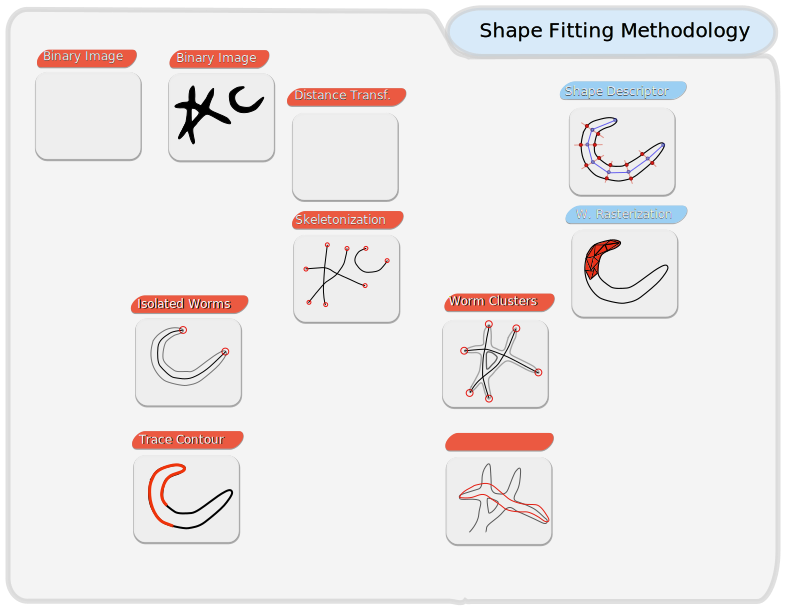
\includegraphics[scale=0.9,angle=270]{diagrams/design.pdf}
 \caption{Descripci\'on gr\'afica de la metodolog\'ia para detectar gusanos C. elegans
   en im\'agenes digitales}
\label{fig:methsol}
\end{figure}

Dada la imagen de entrada, el primer paso consiste en separar los p\'ixeles que
pertenecen a los objetos de estudio (gusanos) del resto de la imagen. Para esto,
se utiliza alg\'un m\'etodo del valor umbral (MVU) que permita calcular una imagen
binaria que separe p\'ixeles de gusanos de los p\'ixeles del fondo. Por lo general,
este proceso no es completamente eficaz, y se obtiene algo de ruido en la imagen, el
cual debe ser eliminado en procesamientos posteriores. Esta primera etapa corresponde
a una segmentaci\'on inicial de la imagen de entrada.
Seguidamente, a partir de la imagen binaria, se puede calcular una transformada de
distancia o mapa de distancias, en la cual se almacena la distancia de cada pixel
al pixel de fondo m\'as cercano. La transformada de distancia hace posible identificar
f\'acilmente los p\'ixeles de contorno en la imagen binaria, lo que la convierte en
una herramienta fundamental para la generaci\'on autom\'atica de perfiles de gusanos,
el trazado de contornos en gusanos aislados y para la optimizaci\'on del proceso
de \emph{esqueletizaci\'on}, entre otros. \\

Habiendo determinado los p\'ixeles que pertenecen a gusanos en la imagen, se pueden separar
los grupos de p\'ixeles que estan conectados y rodeados por p\'ixeles de contorno. Esta
segmentaci\'on provee diversos grupos de p\'ixeles objetos. Cada uno de estos grupos
podr\'ia ser tanto un gusano aislado como una agrupaci\'on de gusanos, de acuerdo a la diferenciaci\'on
expuesta en la Sec. \ref{sec:reasoning}.
Una manera de diferenciar los diferentes grupos es contando el n\'umero de extremos y de intersecciones. 
Un grupo que contiene exactamente dos puntos extremos y que
no presenta intersecciones corresponder\'a a un gusano aislado. Por otro lado, si el grupo presenta
m\'as de dos puntos extremos, o al menos una intersecci\'on, esto indicar\'a la presencia de 
solapamiento de gusanos, por tanto corresponder\'a a una agrupaci\'on de gusanos.\\

El enfoque de ajuste de formas se centra en ubicar inicialmente una silueta de gusano gen\'erica 
cerca de un posible gusano en la imagen. De esta manera, es necesario poder determinar, con cierto grado
de precisi\'on y factibilidad, \'areas que pertenezcan a gusanos individuales en la imagen. Para este prop\'osito,
el esqueleto topol\'ogico de la imagen proveer\'ia un camino continuo a trav\'es del eje medio
de los objetos inicialmente segmentados, conectando puntos extremos de gusanos. Al mismo tiempo, permitir\'ia
detectar gran cantidad de puntos extremos.\\

Seguidamente, los diferentes grupos segmentados son procesados para detectar 
y ajustar la forma de los gusanos individuales que los conforman.
Los dos tipos de grupos definidos (agrupaciones de gusanos y gusanos aislados),
son procesados de formas diferentes. 

\subsubsection*{Gusanos Aislados}
El contorno de la silueta de los gusanos aislados puede ser trazada f\'acilmente de 
la siguiente forma: se selecciona un pixel de contorno (indicado en el mapa de distancias)
y se construye un camino siguiendo el pixel de contorno vecino en cada paso, hasta que
se cierre el contorno. Luego, la silueta puede ser \emph{rasterizada} construyendo 
una maya triangulada y, seguidamente, \emph{rasterizando} cada triangulo por separado. Esto
proveer\'ia el conjunto de los p\'ixeles que pertenecen a la forma del gusano, por lo que
la forma quedar\'ia ajustada.\\
El ajuste cas\'i perfecto que se puede obtener de los gusanos aislados, hace posible
calcular un perfil de gusano que represente a los individuos de la muestra, de forma
general. De esta manera, se puede construir un descriptor de forma preciso (esto 
es explicado a fondo en la secci\'on \ref{sec:metshapedescriptor}).

\subsubsection*{Agrupaciones de Gusanos}
Para detectar los gusanos individuales presentes en una agrupaci\'on de gusanos, 
se calculan las formas de gusanos factibles entre par de puntos extremos y luego 
se determina cuales de aquellas tienen m\'as probabilidades de pertenecer a gusanos 
en la imagen. \\

El proceso en general es como sigue: dado un par de puntos extremos, se selecciona
alg\'un camino entre ellos. Luego, se escogen un conjunto de puntos control y
a partir de estos puntos y del descriptor de forma, 
se genera una silueta de gusano alrededor del camino. Dicho camino constituye el 
eje medio de la silueta generada. Despu\'es de esto, se lleva a cabo un proceso de 
ajuste de formas, que consiste en minimizar la distancia que existe entre la silueta
generada y el gusano que presumiblemente se encuentra dispuesto en un espacio 
cercano al camino escogido, hasta que el mejor ajuste es encontrado. Una forma ajustada,
despu\'es del proceso de minimizaci\'on, se denomina conformaci\'on. Una conformaci\'on 
corresponde a la mejor silueta de gusano que se puede construir a partir de un camino
entre dos extremos determinados, y que presumiblemente representa a un gusano real
de la imagen. \\

Este proceso es repetido para cada camino de gusanos factible que puede ser encontrado
a partir de cada punto extremo. De esta manera, se obtienen todas las conformaciones
posibles en el imagen. Luego, un algoritmo de as\'ignaci\'on permitir\'a seleccionar
el mejor conjunto de conformaciones, que maximice el n\'umero de puntos extremos cubiertos
y minimice el valor acumulado de energ\'ia. Las conformaciones escogidas incorrectamente
a trav\'es de la as\'ignaci\'on autom\'atica, podr\'an ser corregidas siguiendo
un sencillo proceso manual.\\

Un algoritmo de predicci\'on de caminos puede ser utilizado para encontrar
los caminos de gusano m\'as probables, que parten de un punto extremo dado.
Las conformaciones resultantes de los caminos predichos por el algoritmo podr\'ian
ser beneficiados sobre otras conformaciones, para aumentar la probabilidad de que
sean escogidos.\\

En las secciones siguientes se cubren detalladamente los diferentes procesos
involucrados en la metodolog\'ia presentada, y se presenta el enfoque particular
de implementaci\'on seguido en este trabajo, para cada uno de ellos.
  

\subsection{Segmentaci\'on Inicial (M\'etodo del Valor Umbral)}
\label{sec:metthres}

Dado que el prop\'osito principal de este estudio es detectar y ajustar la forma de 
gusanos C. elegans en im\'agenes digitales, un paso inicial fundamental es el de separar
las formas de gusanos lo m\'as posible del resto de la imagen, para as\'i poder llevar a
cabo un an\'alisis m\'as preciso.\\

Sean los gusanos en la imagen los objetos a separar y considerando el resto de la imagen
como fondo o segundo plano, los p\'ixeles de la imagen puede ser separados en dos grupos: 
p\'ixeles de objeto y p\'ixeles de fondo. Dada esta caracterizaci\'on, un m\'etodo del valor
umbral permitir\'ia separar los objetos en la imagen digital y descartar la informaci\'on
innecesaria, representando esto a trav\'es de una imagen binaria. La imagen binaria proveer\'ia
entonces una segmentaci\'on inicial de la imagen original, siendo adem\'as clave para el
c\'alculo del mapa de distancias de la imagen, como se explica en la Sec. \ref{sec:metdt}.
En general, para esta etapa de la metodolog\'ia, cualquier MVU que permita obtener una imagen
binaria que identifique satisfactoriamente los p\'ixeles que pertenecen a los gusanos de la
imagen, ser\'a suficiente para continuar el proceso normalmente, sin importar la existencia
de ruido leve en la imagen.


\subsubsection*{Implementaci\'on}
\label{sec:thresimp}

Existen cuatro MVU para im\'agenes en 2D implementados en \emph{Endrov},
estos son: \emph{Fukunaga}, \emph{m\'axima entrop\'ia}, \emph{Otsu} y \emph{percentil},
que cubren las categor\'ias de MVU basados en histogramas y MVU basados en entrop\'ia 
(ver Sec. \ref{sec:thresholding}). Dada la condici\'on de transparencia de los gusanos
C. elegans, es dif\'icil determinar te\'oricamente cual vendr\'ia a ser el m\'etodo m\'as apropiado 
para obtener una imagen binaria precisa. \\
Por esta raz\'on, se realizaron una serie de experimentos
para seleccionar el m\'etodo m\'as apropiado. Estos experimentos consistieron en el ajuste manual
de los diferentes par\'ametros de cada uno de los m\'etodos mencionados, que fueron aplicados
sobre un conjunto de im\'agenes de prueba. La precisi\'on de segmentaci\'on de las im\'agenes binarias
obtenidas en cada caso, se midi\'o a trav\'es de una comparaci\'on visual con la imagen original.\\
El m\'etodo que mejor se comport\'o en estos experimentos resulto ser el 
\emph{m\'etodo del valor umbral por percentil}, 
al ser el m\'as f\'acil de ajustar manualmente y aquel que retorn\'o el equivalente binario m\'as preciso, 
en cada caso. Un an\'alisis m\'as detallado sobre la escogencia del m\'etodo de valor umbral para esta metodolog\'ia
se presenta en la secci\'on de experimentos del cap\'itulo cuatro (ver Sec. \ref{chap:experiments}).\\

En la figura \ref{fig:wormthres} se presenta una imagen binaria, obtenida al
aplicar el \emph{m\'etodo del valor umbral por percentil}.

\begin{figure}[h t b p ! H]
  \centering
  \subfloat[Imagen original]{\includegraphics[width=0.45\textwidth]{original.png}}
\qquad
  \subfloat[M\'etodo del valor umbral por percentil. Valor=0.074]{\includegraphics[width=0.45\textwidth]{thres/worms}}
\caption{Gusanos en medio l\'iquido. Imagen original e imagen binaria obtenida a trav\'es
del m\'etodo del valor umbral por percentil, con un percentil de 0.074}
  \label{fig:wormthres}
\end{figure}

\subsection{Transformada de Distancia}
\label{sec:metdt}

La transformada de distancia de la imagen binaria es utilizada a fondo en el
seguimiento de contorno y en diferentes tipos de procedimientos de segmentaci\'on.
Espec\'ificamente, el mapa de distancias permite detectar y delinear el contorno
exacto de gusanos aislados (Sec. \ref{sec:metiso}), es \'util en la generaci\'on
autom\'atica de perfiles de gusanos (Sec. \ref{sec:metwormprof}), y es esencial en 
la predicci\'on heur\'istica de caminos de gusanos m\'as probables (Sec. \ref{sec:pathguessing}). 
As\'i mismo, permite mejorar el rendimiento de algoritmo iterativo de reducci\'on de capas
dise\~nado por \emph{Zhang y Suen}, \cite{thinning}, como se describe en 
la Sec. \ref{sec:metsk}

\subsubsection*{Implementaci\'on}
\label{sec:dtimp}

Tal como se describe en \cite[p.196]{fastdt}, los algoritmos para calcular transformadas de distancia pueden ser
categorizados en dos grandes clases: m\'etodos iterativos y m\'etodos secuenciales o recursivos. 
Los m\'etodos iterativos son particularmente eficientes en computadoras de arreglos celulares
dado que se pueden procesar todos los p\'ixeles en paralelo en cada iteraci\'on. Por otro lado, los m\'etodos secuenciales
se ajustan mejor a computadoras convencionales, al evitar iteraciones por ser independientes del tama\~no de los objetos.
Tomando en cuenta los tipos de computadoras a la que tienen acceso la mayor\'ia de las personas que trabajan
en el procesamiento de im\'agenes digitales, los algoritmos secuenciales ofrecen un rendimiento mucho m\'as
eficiente que los iterativos. Por esta raz\'on, se escogi\'o un enfoque secuencial para calcular la 
transformada de distancia de las im\'agenes de entrada. Particularmente se utiliz\'o el algoritmo de
transformaci\'on de dos recorridos con vecindarios de 3x3, presentado en \cite{fastdt}, que es
tanto eficiente como sencillo de implementar.\\

En el trabajo antes mencionado, se describe un algoritmo para calcular el mapa 
de distancias de una imagen en formato de mapa de bits, que consiste en dos recorridos y
una operaci\'on por pixel. La complejidad del algoritmo es $\mathcal{O}(N)$, donde $N$ 
es el tama\~no del arreglo que contiene la imagen.
En dicho trabajo se presenta, inicialmente, un pseudo-c\'odigo para las m\'etricas 
de distancia de \emph{Manhattan} y \emph{tablero de ajedrez}, \cite[p.197]{fastdt}.
Luego, la definici\'on es extendida para mejorar la eficiencia de los c\'alculos 
requeridos para generar un mapa de distancias a trav\'es de la m\'etrica de distancias
\emph{Euclideanas}, \cite[p.198]{fastdt}.
Este algoritmo de dos recorridos, fue implementado utilizando las tres m\'etricas de
distancia mencionadas anteriormente. Esto permite realizar una an\'alisis m\'as amplio
del comportamiento y precisi\'on del proceso de ajuste de formas, al cambiar de
una m\'etrica a la otra. Esto es debido a que los mapas de distancia generados por 
diferentes m\'etricas, representan a los objetos de maneras diferentes, y tienden
a ser sensible a cambios posicionales u otras propiedades. En \cite[p.332]{eucskeleton}
se asegura que las m\'etricas de \emph{tablero de ajedrez} y \emph{Manhattan} son
sensibles a las rotaciones de los objetos, mientras que la m\'etrica \emph{Euclidiana}
permanece invariable ante estas rotaciones; sin embargo, es mucho m\'as costosa de calcular.\\

Dada la forma alargada y estrecha de los gusanos C. elegans, y los diferentes niveles
de precisi\'on que proveen dichas m\'etricas de distancia, es dif\'icil decidir
cual se ajusta mejor al problema de estudio, por lo que debe ser determinado
experimentalmente. La Figura \ref{fig:distance} muestra una imagen binaria y tres
mapas de distancia obtenidos a partir de una imagen que contiene, \'unicamente, un
gusano aislado.

\begin{figure}[h t b p ! H]
  \centering
  \subfloat[Imagen Binaria]{\label{fig:manh}\includegraphics[width=0.35\textwidth]{dt/binary}}
\qquad
  \subfloat[Distancia de Manhattan]{\label{fig:manh}\includegraphics[width=0.35\textwidth]{dt/manhattandt}}
\qquad                
  \subfloat[Distancia de tablero de ajedrez]{\label{fig:chess}\includegraphics[width=0.35\textwidth]{dt/chessboarddt}}
\qquad
  \subfloat[Distancia Euclidiana]{\label{fig:mouse}\includegraphics[width=0.35\textwidth]{dt/euclideandt}}
  \caption{ Imagen binaria y tres mapas de distancia utilizando diferentes m\'etricas,
    a partir de la imagen de un gusano}
  \label{fig:distance}
\end{figure}

\subsection{\emph{Skeletonization}}
\label{sec:metsk}

La \emph{skeletonization} de la imagen corresponde al proceso de obtener un 
camino de p\'ixeles conectado y delgado, que tienda
al eje central o eje medio de los gusanos en la imagen. A este camino se le
denomina esqueleto. Este es un proceso
clave en el enfoque de detecci\'on presentado en este trabajo, tal como
se enuncia inicialmente en la Sec \ref{met:description}. El esqueleto de la
imagen hace posible identificar la cantidad de gusanos presentes, permite
diferenciar y separar las agrupaciones de gusanos de los gusanos aislados, 
y m\'as importante, provee caminos entre extremos de gusanos (que tienden
al eje medio). Estos caminos son fundamentales en el proceso de ajuste
de formas (ver Sec \ref{sec:metsegmentation}), pues proveen informaci\'on
acerca de la localizaci\'on de los gusanos en la imagen, al constituir trayectorias
a lo largo de las cuales podr\'ian estar dispuestos gusanos en la imagen.

\subsubsection*{Implementaci\'on}
\label{sec:skeletonimp}


Para los efectos de este trabajo, el algoritmo de \emph{skeletonization} a ser
seleccionado debe garantizar la conectividad de los puntos del esqueleto, \emph{i.e.}
cada punto del esqueleto debe estar conectado con al menos otro punto del mismo
esqueleto. As\'i mismo, el esqueleto debe ser tan delgado como sea posible 
(hasta un 1 pixel de grosor) para simplificar el procesamiento y an\'alisis de caminos.\\

Existen diferentes m\'etodos que consisten en encontrar los puntos cresta en el
mapa de distancias y conectarlos, como se explica en \cite{maxima,euclideancentre,ridgedt}. 
El enfoque presentado en \cite{maxima} fue seguido inicialmente para calcular un esqueleto
de imagen delgado en un tiempo de ejecuci\'on muy corto. Pese a que el estudio garantiza
que el algoritmo permite calcular, satisfactoriamente, esqueletos conectados de un pixel
de grosor, este result\'o ser eficaz \'unicamente para los gusanos aislados. Los esqueletos
obtenidos para agrupaciones de gusanos resultaron generalmente desconectados, 
de m\'as de un pixel de grosor y poco precisos. Estos llevo a la utilizaci\'on
de un enfoque diferente.\\

En \cite{thinning} se presenta un algoritmo iterativo para calcular el esqueleto de
una imagen binaria. El algoritmo consiste, b\'as\'icamente, en la remoci\'on por capas
de aquellos p\'ixeles que, de acuerdo a determinados criterios, no pertenecen al esqueleto
del objeto. El dise\~no del algoritmo est\'a dirigido a computadoras con procesadores 
paralelos, de manera que se puedan ejecutar varias operaciones de pixel al mismo tiempo,
y mejorar as\'i el rendimiento. Para evitar el requerimiento de utilizar computadores
con procesadores paralelos, sin desmejorar el rendimiento significativamente,
el algoritmo fue ligeramente modificado. Dicha modificaci\'on consiste en utilizar
el mapa de distancias para descartar chequeo de p\'ixeles que pertenecen a capas
m\'as profundas que la capa que est\'a siendo reducida en un momento determinado.
Esto toma ventaja de la naturaleza de los mapas de distancia, quienes, por definici\'on,
establecen capas de distancia entre los p\'ixeles del objeto y el fondo de la imagen.\\
De esta manera, las capas se definen por el valor que tiene cada pixel en el mapa 
de distancias. La primera capa corresponde a un valor de distancia de uno ($1$), la segunda
un valor de dos ($2$) y as\'i sucesivamente. El algoritmo es presentado en \ref{thinninalg}.

\begin{algorithm}                     
\caption{\emph{skeletonization} por reducci\'on por capas}         
\label{thinninalg}                    
\begin{algorithmic}                   
\STATE $pixelesObjeto \leftarrow obtenerPixelesObjetoBinario()$
\STATE $imagenTD \leftarrow calcularTransformadaDistancia()$
\STATE $indiceContorno \leftarrow 1$
\STATE $reducir = True$

\WHILE{$reducir$}

\STATE \COMMENT{eliminar p\'ixeles del borde sur-este y pixel de
esquina nor-oeste}
\FOR{$pixel$ in $pixelesObjeto$}
\IF{$ImagenDT(pixel) > indiceContorno$}
\STATE \COMMENT{saltar iteraci\'on}
\ELSE
\STATE $eliminarPixel \leftarrow condicionSurEste(pixel)$
\IF{$eliminarPixel$}
\STATE $pixelesObjeto.eliminar(pixel)$
\STATE $reducir \leftarrow True$
\ENDIF

\ENDIF
\ENDFOR


\STATE \COMMENT{eliminar p\'ixeles del borde nor-oeste y pixel
esquina sur-este}
\FOR{$pixel$ in $pixelesObjeto$}
\IF{$imagenTD(pixel) > indiceContorno$}
\STATE \COMMENT{saltar iteracion}
\ELSE
\STATE $eliminarPixel \leftarrow condicionNorEste(pixel)$
\IF{$eliminarPixel$}
\STATE $pixelesObjeto.eliminar(pixel)$
\STATE $reducir \leftarrow True$
\ENDIF
\ENDIF
\ENDFOR
\ENDWHILE
\STATE 
\RETURN{$pixelesObjeto$}

\end{algorithmic}
\end{algorithm}

El algoritmo se ocupa bien de los gusanos que se solapan, al construir un camino que 
se aproxima bien al eje central de las figura, y resulta en un esqueleto totalmente
conectado y delgado (mayoritariamente 1-pixel de grosor).
En la Figura \ref{fig:skeleton} se presenta el esqueleto de un conjunto de gusanos.

\begin{figure}[h t b p ! H]
 \centering
   \includegraphics[scale=0.75]{skeleton/skeleton.png}
 \caption{Esqueleto obtenido a trav\'es de reducci\'on por capas iterativa
   de un conjunto de gusanos}
\label{fig:skeleton}
\end{figure} 

\subsection{Segmentaci\'on de Gusanos}
\label{sec:metsegmentation}

Dado que el objetivo es ajustar las formas de gusanos individuales, es 
necesario localizarlos en la imagen y separarlos lo m\'as posible, 
\emph{i.e. }segmentar la imagen. La segmentaci\'on de los objetos 
de estudio permite mejorar la eficiencia y precisi\'on del proceso
de ajuste de formas, al reducir el \'area a analizar, disminuyendo as\'i
la cantidad de combinaciones diferentes que deben ser tomadas en cuenta.
Una vez que se han identificado los puntos extremos, se pueden calcular
los diferentes caminos que existen entre ellos a partir del esqueleto.
A trav\'es del conjunto de puntos extremos y de la cantidad de caminos e 
intersecciones, se puede determinar el tipo de grupo de gusanos al que
pertenece cada grupo de objetos segmentados, ya sean gusanos aislados
o agrupaciones de gusanos. De esta manera, el proceso de ajuste de formas
se puede llevar a cabo en cada grupo por separado.\\

Otro proceso de segmentaci\'on que debe ser llevado a cabo es la identificaci\'on
de caminos de gusanos individuales, tanto para gusanos aislados como para agrupaciones
de gusanos. Estos son caminos que no tiene bifurcaciones y que comienzan y terminan
en puntos extremos.\\
El esqueleto de un gusano aislado determinado corresponde a un camino de este tipo, y es
utilizado para dos procesos diferentes: encontrar el contorno del gusano aislado 
(ver Sec. \ref{sec:metiso}) y generar un perfil de gusanos (ver Sec. \ref{sec:metwormprof}).
El perfil de gusanos permite definir una representaci\'on general de los gusanos en 
la imagen. De esta manera, a trav\'es del perfil y un camino entre dos extremos, se puede
construir una silueta de gusano, que tiene como eje central al camino escogido. \\

Con respecto a las agrupaciones de gusanos, se deben encontrar caminos de gusanos factibles entre
pares de puntos extremos. Si un camino existe entre un par de puntos extremos, ser\'a posible
generar una conformaci\'on de gusano valida a trav\'es del proceso de optimizaci\'on. 
Estos caminos pueden ser escogidos tanto calculando todas las combinaciones de caminos posibles
entre par de puntos extremos, como a trav\'es de un algoritmo de predicci\'on de caminos probables,
como el que se describe m\'as adelante en esta secci\'on.

\subsubsection*{Implementaci\'on}

A continuaci\'on se presentan detalles de la implementaci\'on realizada
de cada uno de los diferentes procesos previamente descritos en esta secci\'on, 
relativos a la segmentaci\'on de gusanos.

\subsubsection*{Puntos Extremos de Gusanos}
\label{sec:wend}

A partir del esqueleto calculado se pueden detectar puntos extremos 
de gusanos. Aquellos p\'ixeles del esqueleto que estan conectados
(son vecinos) de dos o m\'as p\'ixeles se denominan p\'ixeles de cuerpo.
Estos p\'ixeles de cuerpo pertenecen al esqueleto pero no son extremos.
Por otro lado, los puntos extremos del esqueleto son aquellos que estan conectados con
un solo pixel y pueden corresponder al extremo de un gusano, aunque no
necesariamente.\\

Dado que el algoritmo de \emph{skeletonization} basado en reducci\'on por capas
no permite asegurar que los extremos identificados pertenezcan a extremos
de gusanos en la imagen, se debe llevar a cabo un proceso de expansi\'on
del esqueleto, para alcanzar los puntos extremos reales.
El algoritmo se fundamenta en estirar los extremos del esqueleto, siguiendo
una direcci\'on coherente, hasta alcanzar puntos de contorno que vendr\'ian a 
representar los extremos de los gusanos. El algoritmo de expansi\'on utiliza
la definici\'on de \emph{vecino direccional}, que se presenta en \cite[p.334]{maxima}.
Un pixel $D$ es \emph{vecino direccional} de otro pixel $P$, si pertenece a
la vecindad de $P$ (\emph{8-vecindad}) y est\'a localizado dentro de un rango de 
$\pm$ $45^{\circ}$  de cambio de pendiente, con respecto a la orientaci\'on actual
del camino recorrido hasta $P$. En la Figura \ref{fig:directional} se presentan 
tres ejemplos de vecindades direccionales.\\
El algoritmo consiste en seguir el mejor camino direccional, partiendo de cada
punto extremo y expandiendo el esqueleto, hasta que un punto de contorno es
encontrado.
 
\begin{figure}[h t b p ! H]
 \centering
   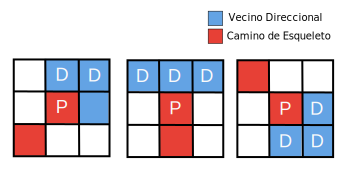
\includegraphics[scale=1]{skeleton/directional.pdf}
 \caption{Tres vecindades direccionales}
 \label{fig:directional}
\end{figure}

El algoritmo de expansi\'on de esqueleto puede ser resumido en 
los siguientes pasos:

\begin{itemize}
\item Seleccionar un punto extremo.
\item Encontrar el pixel de esqueleto anterior y calcular la
  vecindad direccional.
\item Seleccionar el vecino direccional con el menor valor en el
  mapa de distancia y marcarlo como pixel de esqueleto.
\item Si el vecino seleccionado no es un punto de contorno, repetir
  el proceso.
\end{itemize}

Seguidamente se lleva a cabo un proceso de remoci\'on de p\'ixeles de objeto 
incorrectos, que consiste en eliminar aquellos esqueletos cuyo tama\~no (en 
cantidad de p\'ixeles) sea menor que un umbral determinado. Esto permite remover
regiones ligeramente ruidosas, as\'i como punto extremos incorrectos.
Una vez que el esqueleto ha sido expandido satisfactoriamente, los puntos
extremos del esqueleto son marcados como puntos extremos de gusanos.\\

Es importante considerar que, en algunos casos, hay puntos extremos de gusanos
que no puede ser detectados a trav\'es del proceso previamente descrito. 
Particularmente en im\'agenes con gran cantidad de gusanos, donde existe
una alta posibilidad de que los solapamientos entre gusanos oculten
puntos extremos. Para solucionar esto, se puede llevar a cabo un proceso
manual de adici\'on de puntos extremos faltantes, como se explica en 
la Sec. \ref{sec:manualproc}.


\subsubsection*{Segmentaci\'on en Grupos}


Habiendo detectados los puntos extremos de los diferentes grupos de esqueletos
en la imagen, se puede identificar a qu\'e tipo de grupo de gusano corresponde cada uno:
ya sea agrupaciones de gusanos o gusanos aislados. Esto se hace identificando
los extremos de gusanos que estan unidos a trav\'es de un camino del esqueleto.
Como se explic\'o previamente, los gusanos que se superponen son considerados 
parte de un objeto en com\'un en la imagen binaria, por lo que los puntos
extremos que pertenecen a los esqueletos de agrupaciones de gusanos se encuentran
conectados a trav\'es de un camino del esqueleto.\\

Basado en este razonamiento, se dise\~n\'o un algoritmo que detecta la cantidad de
puntos extremos que son conectados a trav\'es de caminos de un determinado esqueleto,
y determina el tipo de grupo de gusanos al que pertenece. Aquellos esqueletos donde
se conectan exactamente dos puntos extremos a trav\'es de uno y solo un camino, corresponde
a gusanos aislados. Mientras que los esqueletos en donde m\'as de dos puntos extremos son
conectados corresponden a agrupaciones de gusanos.
Este procedimiento es descrito en los Algoritmos \ref{groupsegment} y \ref{groupsegment2}.

\begin{algorithm}[h]                     
\caption{Segmentaci\'on en grupos de gusanos}         
\label{groupsegment}                    
\begin{algorithmic}                   

\STATE $listaPtsExt \leftarrow$ lista de puntos extremos
\STATE $indiceAgrupacion \leftarrow$ 0
\FOR{$ptExtremo$ in $listaPtsExt$}
\IF{$ptExtremo.visitado()$}
\STATE \COMMENT{saltar iteraci\'on}
\ELSE
\STATE $indiceAgrupacion +=1$
\STATE $segmentarPorCaminos(ptExtremo,indiceAgrupacion)$
\ENDIF
\ENDFOR
\end{algorithmic}
\end{algorithm}

\begin{algorithm}[h]                     
\caption{Seguimiento de caminos para segmentaci\'on ($segmentarPorCaminos(ptActual,clusterCount)$ )}         
\label{groupsegment2}
\begin{algorithmic}                   

\REQUIRE $ptActual$
\REQUIRE $indiceAgrupacion$

\IF{not $ptActual.esPuntoEsqueleto()$}
\RETURN 
\ELSE
\STATE $agregar(ptExtremo,indiceAgrupacion)$
\ENDIF

\STATE \COMMENT{continuar siguimiento de camino}
\IF{$ptActual.esPtExtremo()$}
\STATE $marcarPtExtremoVisitado(ptActual)$
\ENDIF
\STATE $vecinos \leftarrow obtenerVecindad()$
\FOR{$v$ in $vecinos$}
\STATE $followPath(v,indiceAgrupacion)$
\ENDFOR

\end{algorithmic}
\end{algorithm}


\subsubsection*{Predicci\'on de Caminos}
\label{sec:pathguessing}

Una agrupaci\'on de gusano es definida por un esqueleto
que conectan puntos extremos a trav\'es de caminos. Sin embargo, hasta esta etapa,
se desconoce el par de puntos extremos que pertenecen a cada gusano en la imagen, y 
el mejor camino en el esqueleto
que conecte a cada par, y que mejor represente el eje central de cada gusano 
respectivo.\\

El algoritmo de optimizaci\'on, cubierto en la Sec. \ref{sec:metfit}, lleva a cabo un
proceso de manipulaci\'on de siluetas para ajustar formas de gusanos en la imagen, dados
dos puntos extremos y un camino que los conecte. Para calcular la forma de gusano m\'as probable
que parte de un punto extremo determinado, el algoritmo tendr\'ia que probar cada camino posible
que parte de dicho punto extremo y seleccionar el que mejor se ajuste, lo que tiende a traducirse  
en un alto costo en tiempo de ejecuci\'on.\\
Con el fin de reducir el tiempo de ejecuci\'on del algoritmo de ajuste de
formas, y as\'i mismo proveer un par\'ametro adicional para determinar la
factibilidad de los caminos analizados, se desarroll\'o un algoritmo de
predicci\'on de caminos. En s\'intesis, el algoritmo lleva a cabo una b\'usqueda
heur\'istica para determinar aquellos caminos que tienen mayor probabilidad
de representar a un gusano de la imagen.\\

El algoritmo de predicci\'on se basa en la idea de evitar caminos que
tienden a describir conformaciones no-naturales de gusanos. Para esto
es necesario identificar cambios abruptos en el camino y flexiones
poco comunes o imposibles en gusanos. La idea desarrollada para lograr
esto se centra en que cada paso siguiente que sea seleccionado, corresponda
a la direcci\'on m\'as coherente con respecto al camino que ha sido
trazado hasta ese momento. 
M\'as espec\'ificamente, se escoge el conjunto $S$ de los \'ultimos $N$ 
pasos trazados, y a partir de este, se calcula la direcci\'on m\'as com\'unmente
seguida en esa porci\'on del recorrido.\\

Una dificultad considerable que surge de este
enfoque, es que el seguimiento del camino tiende a evitar \emph{centros de bifurcaciones}.
Una bifurcaci\'on ocurre cuando m\'as de un camino diferente puede ser seguido a partir
de un punto determinado. Dado que estas bifurcaciones son originadas por solapamiento 
de gusanos, el \'area de la bifurcaci\'on suele ser grande, y por tanto hay mayor 
cantidad de p\'ixeles posibles a escoger como siguiente paso. Los \emph{centros de bifurcaciones}
son aquellos puntos que se ubican en la zona m\'as c\'entrica de estas \'areas, y por tanto
se encuentran a una distancia normalmente similar de todos los caminos que se bifurcan.
Para poder determinar con mayor precisi\'on el camino m\'as adecuado a seguir, el trazado del camino 
debe tender a los \emph{centros de bifurcaciones}. Sin embargo, siguiendo el enfoque presentado, estos
centros se tienden a bordear. Por esta raz\'on se desarroll\'o una heur\'istica, que permita
al recorrido tender hacia los \emph{centros de bifurcaciones} y llevar as\'i a una 
decisi\'on mejor informada.\\

La heur\'istica consiste b\'as\'icamente en considerar el valor en el mapa de distancias
del pixel elegible, multiplicado por un factor de equilibrio. De esta manera, la 
selecci\'on del pixel siguiente se basa en dos valores fundamentales: la cantidad
de veces que ha sido escogida la direcci\'on en la que se encuentra dicho pixel, 
en los \'ultimos $N$ pasos, y el valor de la heur\'istica para ese pixel. Esto
puede expresarse de la siguiente forma:

$$Siguiente(p) = \max_{s \in vecindad(p)} (valorDir(direccion(p,s),N) + td(n)*factorH)$$

donde $p$ es el \'ultimo pixel marcado, $valorDir$ es una funci\'on que calcula
la cantidad de veces que la direcci\'on del pixel vecino $s$ ha sido escogida, $td$ es el 
mapa de distancia y $factorH$ es el factor heur\'istico que controla la influencia 
del mapa de distancia.\\


El Algoritmo \ref{guess} presenta un pseudo-c\'odigo para este enfoque de predicci\'on
de caminos de gusanos.

\begin{algorithm}[h]                    
\caption{Pseudo c\'odigo: Algoritmo de predicci\'on de caminos}
\label{guess}                    
\begin{algorithmic}                   

\STATE $listaPtsExtremos \leftarrow$ lista de puntos extremos
\STATE $longitud \leftarrow$ longitud estimada de gusanos multiplicada por un factor escalar
\FOR{$puntoExtremo$ in $listaPtsExtremos$}
\IF{$alcanzado(puntoExtremo)$}
\STATE \COMMENT{saltar iteracion}
\ENDIF
\STATE{$marcarComoAlcanzado(puntoExtremo)$}

\STATE $camino \leftarrow$ lista vacia

\STATE $extremoAlcanzado \leftarrow False$
\STATE $pixelActual \leftarrow puntoExtremo$
\WHILE{$not(extremoAlcanzado)$ and $size(path)<longitud$}
\STATE $pixelActual \leftarrow obtenerMejorVecino(pixelActual)$
\STATE $actualizarArregloDirecciones(direccion(pixelActual))$
\STATE $camino.agregar(pixelActual)$
\IF{$esPuntoExtremo(pixelActual)$}
\STATE $extremoAlcanzado \leftarrow True$
\ENDIF
\ENDWHILE 

\ENDFOR

\end{algorithmic}
\end{algorithm}

\subsection{Descriptor de Forma}
\label{sec:metshapedescriptor}

Como se mencion\'o inicialmente en la Sec. \ref{met:description}, 
el enfoque metodol\'ogico dise\~nado se basa en la manipulaci\'on de 
siluetas de gusanos que se generan a partir de un descriptor de forma.
La forma de un gusano puede ser descrita en t\'erminos geom\'etricos
como objetos alargados, delgados y cil\'indricos. Dado que el proceso
de \emph{skeletonization} y la posterior segmentaci\'on de la imagen, hacen
posible obtener caminos entre pares de extremos de gusanos, un descriptor
de forma permitir\'ia construir siluetas de gusanos a lo largo del
eje central definido por el camino, lo que servir\'ia como par\'ametro
de entrada para el algoritmo de ajuste de formas.\\


El descriptor fue dise\~nado bas\'andose en la idea de generar una silueta
de gusano representativa alrededor del eje central. El descriptor consiste en
dos elementos principales: un conjunto de puntos control y un perfil de gusano.
El conjunto de puntos control est\'a conformado por $N$ puntos equidistantes a lo
largo del eje central del gusano definido por el esqueleto, incluyendo los
dos puntos extremos. Por su parte, el perfil de gusano define $N$ valores de 
grosor que son asociados a cada punto control, respectivamente. El grosor de
un punto control determinado representa el radio de la circunferencia que tiene
como centro a dicho punto. De esta manera, seleccionando dos puntos en posiciones
opuestas de la circunferencia de grosor de capa punto control, y uniendo luego estos
puntos a trav\'es de una curva suave, se obtiene una contorno
que modela la silueta del gusano, como se muestra en la Figura 
\ref{fig:descriptor}. 

\begin{figure}[h]
 \centering
   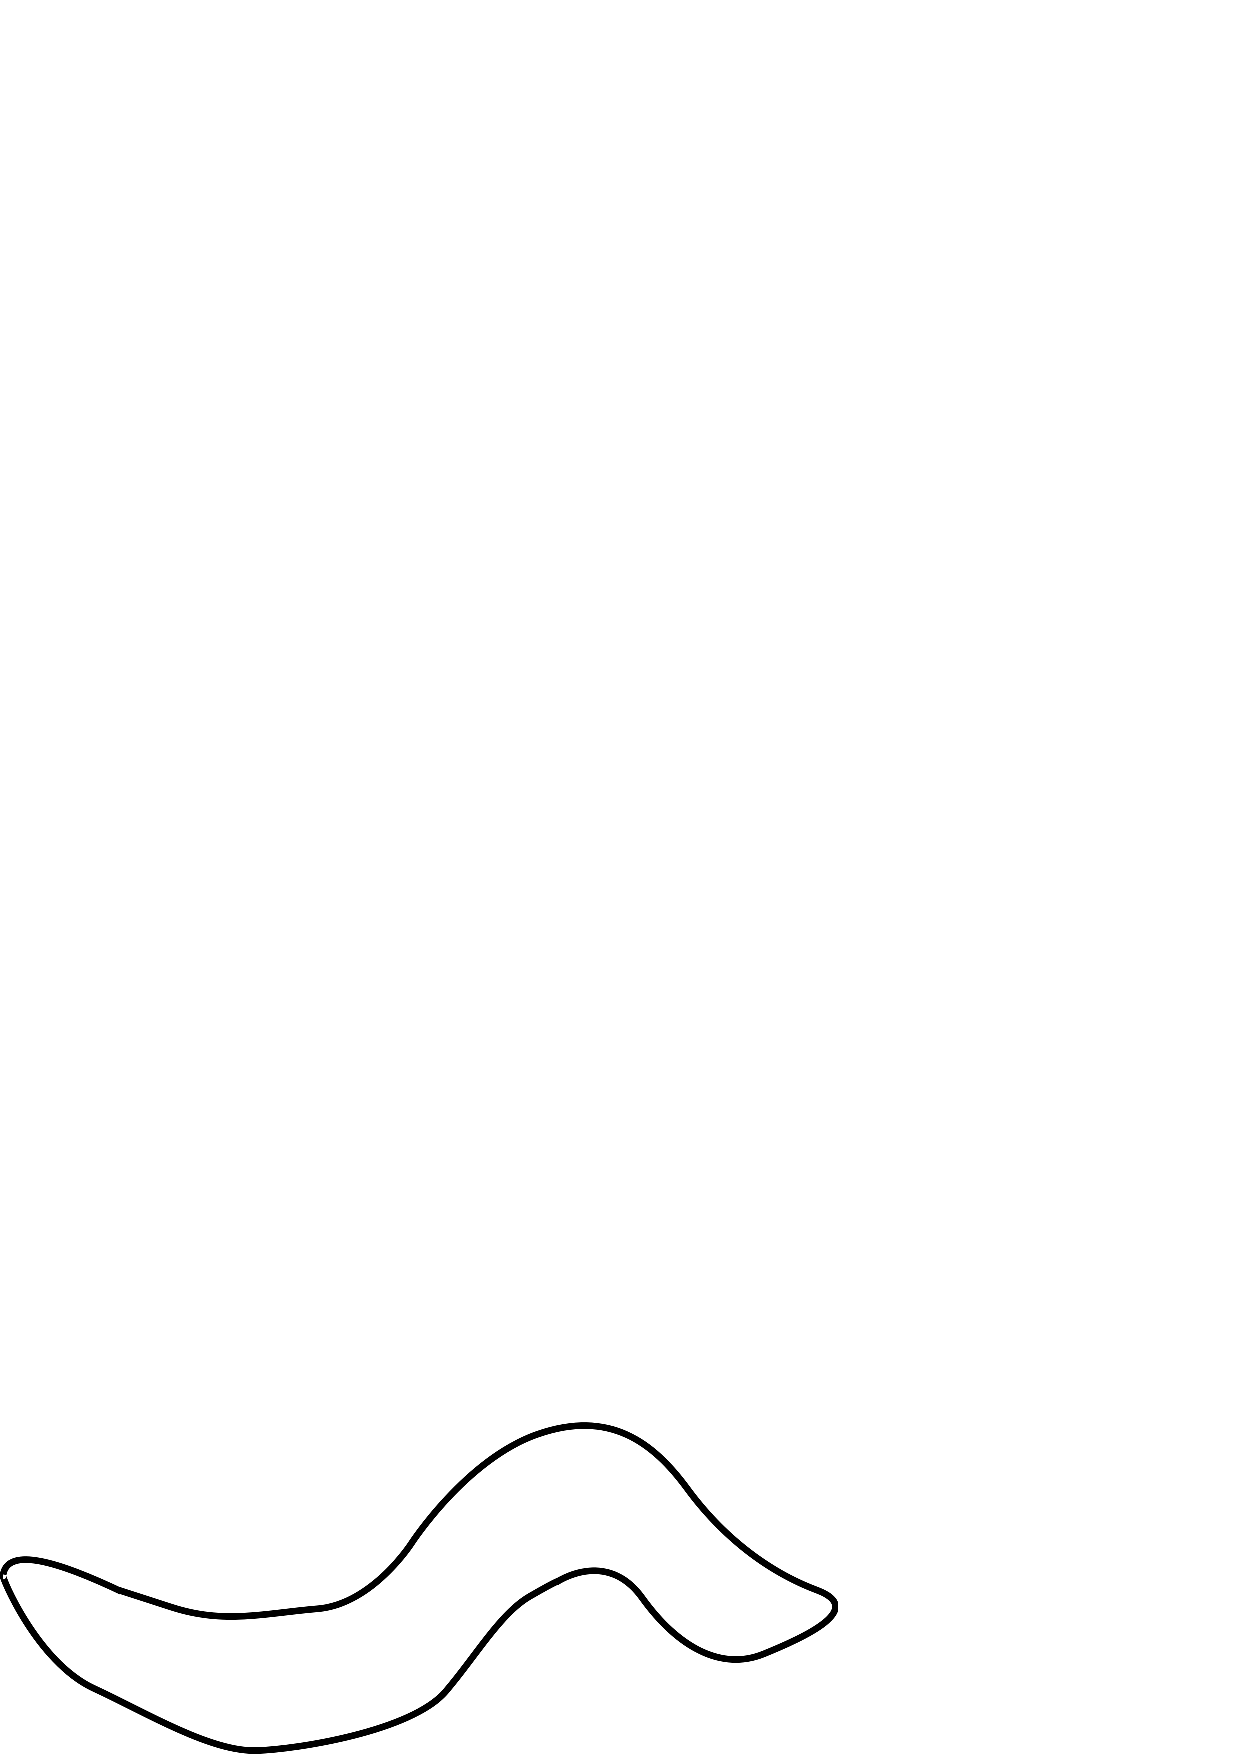
\includegraphics[scale=1]{descriptor/descriptor-vector.pdf}
 \caption{Construcci\'on de una forma de gusano basada en un descriptor de forma}
 \label{fig:descriptor}
\end{figure}

Para obtener un contorno que represente una forma de gusano de manera precisa,
la escogencia de los puntos opuestos en las circunferencias de grosor
debe tomar en cuenta las flexiones del esqueleto. Dado que el contorno se
construye de acuerdo al grosor de los puntos control, las flexiones del gusano
a representar ocurren en cada uno de los puntos control. El grado de flexi\'on
de cada punto control se calcula como el \'angulo que existe entre las rectas
que conectan dicho punto con el punto anterior y posterior, respectivamente.\\

Por cada punto control, se calcula la bisectriz del \'angulo de flexi\'on y luego
se marcan los dos puntos opuestos donde se intersecan la bisectriz y la circunferencia
de grosor. Al calcular una curva que pasa por todos estos puntos, se obtiene un
contorno suave que modela una forma de gusano.\\

Generar una curva suave alrededor de los puntos control mejora la precisi\'on
de la forma descrita, en comparaci\'on con trazar l\'ineas rectas que
conecten los puntos de contorno. Esta representaci\'on permite modelar el 
contorno con m\'as detalle, utilizando un cantidad considerablemente menor
de puntos. La curva suave es obtenida calculando un \emph{spline} cardinal
(ver Sec. \ref{sec:splines}) dados los puntos contorno.\\

El perfil de gusanos para un conjunto de puntos control de tama\~no determinado 
puede ser, tanto definido manualmente, como calculado autom\'aticamente a partir
de los gusanos aislados, como se explica en el siguiente punto.


\subsubsection*{Generaci\'on Autom\'atica de Perfiles}
\label{sec:metwormprof}

La forma de los gusanos aislados puede ser ajustada con precisi\'on, siguiendo
los puntos de contorno en el mapa de distancia, como se explica en la Sec. \ref{sec:metiso}.
Dado un conjunto de formas ajustadas de gusanos aislados y sus esqueletos respectivos, se 
puede generar un perfil de gusanos, midiendo el grosor de los puntos control y calculando
la media aritm\'etica de cada uno.\\

Para medir el grosor de cada punto control, se selecciona inicialmente un conjunto
de $N$ puntos equidistantes que cubren el esqueleto de un gusano aislado determinado.
Seguidamente, como se describe en la secci\'on previa, se calculan las bisectrices de los \'angulos
que existen entre las rectas que conectan los puntos control. A partir de cada punto control, 
se recorren los p\'ixeles de la bisectriz hasta que un punto de contorno es encontrado. Este
recorrido se hace en los dos sentidos, por lo que el proceso devuelve dos puntos de contorno.
A continuaci\'on, se calcula la distancia Euclidiana que existe desde cada punto control hasta
sus dos puntos opuestos respectivos, y se almacena el promedio de distancia.\\

Al repetir este proceso para cada gusano aislado se generan un conjunto de perfiles de gusanos
aislados, uno por cada gusano. A partir de este conjunto de perfiles, se calcula un perfil
general encontrando la media aritm\'etica de los valores de grosor por cada punto control.\\
Para que el perfil sea lo m\'as representativo posible, se descartan el $20\%$ de los gusanos
m\'as grandes y m\'as peque\~nos. El valor de grosor para los puntos extremos, \emph{i.e.} el
primer y \'ultimo punto en el conjunto de tama\~no $N$, es cero, por lo que en los extremos
solo se genera un punto de contorno, en vez de dos como en el resto de los puntos control.\\

Este proceso permite calcular entonces un perfil de grosor que define la distancia 
promedio de cada punto control a su punto de contorno m\'as cercano, haciendo posible
la generaci\'on de siluetas gen\'ericas de gusano alrededor de cualquier esqueleto.

\subsection{Rasterizaci\'on de Siluetas}
\label{sec:metrast}

El enfoque de ajuste de formas se centra en minimizar la distancia entre siluetas
generadas y las formas de gusanos en la imagen. Para medir esta distancia se debe 
conocer el \'area de la silueta que es deformada.\\
El \'area de la silueta puede ser calculada a partir de su contorno. En t\'erminos
del tipo de datos que aqu\'i se manejan, el \'area consiste en el conjunto de p\'ixeles
que son cubiertos por la silueta, incluyendo los p\'ixeles de contorno.\\

El enfoque seguido para calcular el \'area consiste en dividir
en tri\'angulos el espacio definido por el contorno cerrado de la silueta y luego
rasterizar cada tri\'angulo por separado. El t\'ermino rasterizar se
refiere al proceso de transformar una imagen descrita en t\'erminos vectoriales
en un conjunto de p\'ixeles, de manera que pueda ser visualizada.\\

La descomposici\'on de un pol\'igono en tri\'angulos simples, es un problema
cl\'as\'ico de computaci\'on gr\'afica. Diversas soluciones se han propuesto
como lo son: triangulaci\'on de Delaunay, triangulaci\'on de costo m\'inimo y
m\'etodo de \emph{ear clipping}, entre otros.
 
\subsubsection*{Implementaci\'on}

El m\'etodo de \emph{ear clipping} fue escogido por su capacidad para triangular pol\'igonos
c\'oncavos y su sencillez de implementaci\'on. Para convertir el contorno del gusano en un 
pol\'igono, se transforma el \emph{spline} que lo define en un conjunto discreto de puntos.
Cada punto sucesivo es conectado a trav\'es de rectas, definiendo un pol\'igono cerrado. 
Para que la representaci\'on poligonal no afecte la suavidad del contorno definido por el
\emph{spline}, se escogen los puntos discretos (p\'ixeles) lo m\'as cerca posible uno de otros.
Seguidamente el contorno poligonal es triangulado.\\

Cada tri\'angulo es \emph{rasterizado} siguiendo el algoritmo de rasterizaci\'on por barrido
explicado en \cite{scanconversion}. El algoritmo consiste en rasterizar 
l\'ineas horizontales entre los lados del triangulo hasta que el \'area es cubierta por completo.\\

Una vez \emph{rasterizados}, se pueden almacenar el \'area y el contorno de la silueta en
forma de datos manejables y visualizables. 

\subsection{Detecci\'on y Ajuste de Formas}
\label{sec:metfit}

Una vez que la imagen ha sido segmentada en diferentes grupos de gusanos; que se tiene
el esqueleto que representa el eje central de dichos grupos; y que se ha calculado un
perfil general de los gusanos en la imagen, se puede llevar a cabo el proceso de ajuste
de formas. Este proceso permite detectar los gusanos individuales que componen los 
diferentes grupos y almacenar sus formas respectivas en forma datos manejables y visualizables.\\

El proceso de detecci\'on y ajuste es diferente para cada tipo de grupos de gusanos: 
gusanos aislados y agrupaciones de gusanos. En esta secci\'on se explican las 
caracter\'isticas de este proceso en cada caso.

\subsubsection*{Ajuste de Formas en Gusanos Aislados}
\label{sec:metiso}

En esta etapa de la metodolog\'ia, se conocen los diferentes gusanos aislados
y se tiene, por cada uno, un esqueleto delgado que conecta dos puntos
extremos de gusano a trav\'es de un camino.
Dado que este proceso es llevado a cabo despu\'es de que cada punto extremo
ha sido identificado correctamente y se conoce que el esqueleto no tiene
bifurcaciones, el \'area conformada por los p\'ixeles objeto del grupo
segmentado corresponder\'an a la forma exacta del gusano aislado en la
imagen.\\

Con el prop\'osito de tener una informaci\'on m\'as amplia acerca de los gusanos
detectados, se calcula tambi\'en el contorno a partir del \'area previamente identificada.
El contorno es trazado encontrando el pixel de borde m\'as cercano a alg\'un punto extremo
del gusano y recorriendo cada pixel de contorno vecino hasta cerrar el camino. 
Un pixel de contorno es aquel que tiene el valor de uno (1) en el mapa de distancias.\\

Este proceso permite, entonces, obtener el contorno y el \'area de cada
gusano aislado en la imagen, de manera precisa.

\subsubsection*{Ajuste de formas en Agrupaciones de Gusanos}
\label{sec:clusterfit}

Las agrupaciones de gusanos representan un escenario de detecci\'on m\'as complicado, 
debido a la cantidad variable de gusanos que los conforman y el solapamiento entre estos.
El solapamiento entre gusanos hace dif\'icil diferenciar el conjunto de p\'ixeles que pertenecen
al \'area de un gusano u otro. Por esta raz\'on, se dise\~n\'o un proceso de ajuste de formas
que se encarga de calcular las conformaciones o formas de gusanos factibles que parten
de cada punto extremo, para luego determinar el conjunto de conformaciones que mejor
ajustan la agrupaci\'on de gusanos como un todo.\\

El ajuste de formas sigue un enfoque de optimizaci\'on basado en la minimizaci\'on
de distancias entre gusanos de la agrupaci\'on y siluetas gen\'ericas, que son deformadas
para ajustarse a ella. Por lo tanto, una conformaci\'on de gusano es obtenida cuando
la disimilitud entre una silueta deformada y un \'area determinada de la agrupaci\'on, 
es la m\'inima posible.\\

A continuaci\'on, se describen los pasos y caracter\'isticas principales de este proceso:


\begin{itemize}
\item Por cada punto extremo se calcula el conjunto de caminos del esqueleto factibles
que comienzan en ese extremo.
\item Dado un camino del esqueleto, se construye una silueta gen\'erica a trav\'es
del descriptor de forma y el perfil de gusanos en la imagen. La silueta es dispuesta
a lo largo del camino.
\item Un proceso de optimizaci\'on se encarga de deformar la silueta hasta que la
disimilitud (distancia) entre dicha silueta y la imagen binaria es minimizada. Una
vez optimizada, la silueta corresponder\'a a una conformaci\'on de gusano factible.
\item Una vez que se han calculado todas las posibles conformaciones que parten 
de cada punto extremo, se selecciona el conjunto de conformaciones que maximiza
el n\'umero de puntos extremos cubiertos y minimiza el valor de distancia acumulado.
Las conformaciones seleccionadas corresponden a los mejores ajustes que se pueden
obtener de forma autom\'atica.
\item Las conformaciones escogidas que no representan a un gusano real en la imagen
(conformaciones incorrectas) pueden ser corregidas a trav\'es de un sencillo proceso
manual.
\end{itemize}

\subsubsection*{Deformaci\'on de Siluetas}
\label{sec:defsil}

Los caminos del esqueleto que son calculados (que van de un punto extremo a otro), 
corresponden a aproximaciones de posibles esqueletos de gusanos en la imagen. 
Dado que el modelo a deformar se construye sobre un camino del esqueleto
(que tiende al eje medio de un \'area de la agrupaci\'on de gusanos), la 
silueta generada inicialmente se encontrar\'a siempre cerca de una forma
de gusano real. Dado esto, a trav\'es de perturbaciones simples y ligeras de la silueta generada, 
se podr\'a deformar el modelo lo suficiente como para corregir la desviaci\'on del
esqueleto con respecto al eje central real del gusano a ajustar. De esta manera, se permite obtener  
la forma de gusano mejor aproximada que se puede calcular a partir del camino dado.\\

La deformaci\'on de la silueta se hace a trav\'es del descriptor de forma, que se 
encuentra definido por un conjunto de puntos control. Con el objetivo de proveer
formas de gusano factibles y para limitar la cantidad de deformaciones posibles,
una deformaci\'on consistir\'a en el reposicionamiento de un punto control.
La cantidad de posiciones diferentes que un punto control puede tomar es fija,
y son dispuestas a lo largo de la bisectriz del \'angulo del punto control. 
Este \'angulo depende, a su vez, de la posici\'on de los otros puntos control.\\
Siguiendo esto, se puede obtener un gran conjunto de deformaciones posibles
de forma r\'apida.

\subsubsection*{Funcional de Energ\'ia}
\label{sec:energyformulation} 

La funci\'on de distancia debe proveer una medida de que tan bien se aproxima la silueta que se
deforma a un gusano en la imagen, \emph{i.e.} que tan bien se ajusta la forma deformada.
Para esto se utiliz\'o el concepto de funcional de energ\'ia, tal como se define
en el modelo de contornos activos, \cite{snakes}.\\

El funcional de energ\'ia describe la distancia entre el modelo que se deforma 
y la imagen, y gu\'ia el proceso de ajuste de contornos. De esta manera, mientras menor
sea el valor devuelto por el funcional de energ\'ia, menor es la distancia y por tanto
mejor se ajusta el modelo. El funcional es formulado en base a dos 
conceptos: la energ\'ia externa y la energ\'ia interna. La suma de los valores
de la energ\'ia externa e interna relativas a un modelo, constituye el valor
de energ\'ia para ese modelo espec\'ifico.\\

La energ\'ia externa describe que tan bien se ajusta el modelo deformado a la 
imagen. Conociendo que, mientras mayor es la cantidad de p\'ixeles de fondo que son cubiertos 
por el modelo m\'as alejado se encuentra el modelo de un gusano en una agrupaci\'on, 
una medida apropiada para la energ\'ia interna ser\'ia 
la proporci\'on de p\'ixeles de fondo que son cubiertos por el modelo deformado.
De esta manera, mientras mayor es la cantidad de p\'ixeles de objeto 
que son cubiertos, menor es el valor de la energ\'ia externa.
Por lo tanto, dado un modelo $M$ y la funciones $bg$ y $fg$ que miden la cantidad
de p\'ixeles de fondo y de objeto que cubre el modelo, respectivamente, se puede
definir la energ\'ia externa para este problema de la siguiente forma:

$$E_{ext}(M) = \frac{bg(M)}{bg(M)+fg(M)}$$

Otra posibilidad consistir\'ia en tomar en cuenta, \'unicamente, la cantidad
de p\'ixeles de fondo. Sin embargo, dado la variabilidad de la cantidad de p\'ixeles
que puede cubrir una silueta de gusano, esta medida causar\'ia a la energ\'ia externa
ser muy variable de una silueta a otra.\\

La energ\'ia interna modela la resistencia de la silueta (modelo) a perder, a trav\'es
de la deformaci\'on, las caracter\'isticas que la hacen representar a la clase que
modela, \emph{e.g.} la clase de gusanos. Esto significa que, para el problema que aqu\'i
se aborda, la energ\'ia interna modelar\'ia la resistencia de la silueta de gusano
a ser deformada de manera tal que dejase de ser representativa de un gusano.
Como se explica en \cite{snakes}, la energ\'ia interna funciona como una restricci\'on de 
suavidad de los contornos del modelo y se formula de forma expl\'icita (normalmente en
t\'erminos diferenciales). Sin embargo, en el enfoque propuesto en este trabajo,
cada silueta a deformar se genera a partir de un perfil de gusano ajustado a un
descriptor de forma, por lo que cada silueta generada pertenece inequ\'ivocamente
a la clase de siluetas de gusano. Por esta raz\'on no es necesario incluir la
energ\'ia interna en el funcional de energ\'ia.

\subsubsection*{Optimizaci\'on}

A trav\'es del  proceso de optimizaci\'on se desea obtener las conformaciones de gusanos factibles
dentro de una agrupaci\'on de gusano. El enfoque general se basa en producir siluetas gen\'ericas
a partir de los caminos del esqueleto que conectan puntos extremos de gusanos, y deformarlas
levemente de manera que se ajusten a la imagen lo mejor posible. 
Una vez que se tiene un descriptor de formas basado en el esqueleto 
(Sec. \ref{sec:metshapedescriptor}), un m\'etodo de deformaci\'on de siluetas 
(Sec. \ref{sec:defsil}) y una funci\'on objetivo que modele la distancia
entre las siluetas y la agrupaci\'on a ajustar (Sec. \ref{sec:energyformulation}), 
s\'olo basta escoger un m\'etodo de optimizaci\'on.\\

De acuerdo al enfoque que aqu\'i se presenta, se puede utilizar cualquier m\'etodo de 
optimizaci\'on que permita minimizar la funci\'on objetivo que define la distancia entre 
formas de gusanos, a partir de una soluci\'on factible inicial, que, a su vez, permite 
generar otras soluciones factibles a trav\'es de un m\'etodo de deformaci\'on.\\

Dado lo r\'apido que pueden ser calculados grandes conjuntos de deformaciones,
de acuerdo al enfoque presentado en la Sec. \ref{sec:defsil}, se escogi\'o
una meta heur\'istica de b\'usqueda local como m\'etodo de optimizaci\'on.
El proceso en general consiste en obtener el mejor individuo de la vecindad
que mejore el valor del funcional de energ\'ia, hasta que la funci\'on sea
minimizada.\\
La vecindad es calculada de la siguiente manera:
Para una silueta determinada, se efect\'uan cuatro deformaciones diferentes por cada punto
control. Particularmente, dos en cada una de las dos direcciones opuesta de la bisectriz
del punto control. Existen entonces $(N-2)*4$  
deformaciones posibles (vecinos) por cada silueta \footnote{Los puntos control que corresponden 
a los extremos permanecen fijos. Por eso el n\'umero de puntos control tomados en cuenta es $N-2$}, 
donde $N$ es el n\'umero de puntos control. De esta manera, una vecindad consiste en deformaciones
leves y ligeramente m\'as fuertes de una silueta de gusano para cada punto control.\\ 
Los puntos control que corresponden a los extremos del esqueleto permanecen fijos.\\

Una vez que la mejor silueta es obtenida, se lleva a cabo un proceso de correcci\'on
de contornos. Este proceso consiste en la expansi\'on o contracci\'on de determinadas 
secciones del contorno de la silueta, para adaptarla al gusano real de la imagen.
Esto es requerido dado que la silueta optimizada es generada inicialmente siguiendo un 
perfil de gusano, el cual representa la forma de los gusanos de una manera gen\'erica, y
por tanto no describe las formas exactas de los gusanos en la imagen.\\
En este proceso, los puntos de contorno construidos a partir de los puntos control son
empujados hacia puntos de contorno de la imagen, de acuerdo al mapa de distancias, ya
sea expandi\'endolos o contray\'endolos. Cada posici\'on nueva considerable para el punto
contorno debe poseer un valor en el mapa de distancia similar o menor al que pose\'ia
originalmente.

\subsubsection*{Selecci\'on de Conformaciones}

Despu\'es que el proceso de optimizaci\'on es llevado a cabo, se debe seleccionar
un subconjunto de conformaciones por cada agrupaci\'on de gusano, que representar\'a
la as\'ignaci\'on final de conformaciones y por tanto la soluci\'on encontrada al final
del proceso. El subconjunto seleccionado debe maximizar la cantidad
de puntos extremos cubiertos y minimizar la suma de las energ\'ias finales de
cada conformaci\'on (valor minimizado de la funci\'on objetivo).\\

Cada punto extremo debe corresponder como m\'aximo a una conformaci\'on. De esta
manera, a cada punto extremo le corresponde uno y s\'olo uno de los otros puntos extremos.
Por consiguiente, el subconjunto \'optimo de conformaciones corresponder\'a a la
as\'ignaci\'on de costo m\'inimo (energ\'ia de cada conformaci\'on) entre el 
conjunto de puntos extremos, por cada agrupaci\'on de gusano.\\

Esta as\'ignaci\'on puede ser resuelta resolviendo el problema de as\'ignaci\'on de
costo m\'inimo de un grafo no-bipartito. Sin embargo, dado la complejidad de
su implementaci\'on (y posible sobrecarga en rendimiento) de este algoritmo,
se dise\~n\'o una soluci\'on diferente, consistiendo en un algoritmo \emph{greedy}
iterativo. El algoritmo es aplicado a subgrupos de agrupaciones de gusanos.
Estos sub grupos estas comprendidos, \'unicamente, por puntos extremos que estan
conectados por caminos factibles. Los puntos extremos que pertenecen a subgrupos
ser\'an llamados puntos conflictivos.\\

El algoritmo consiste en lo siguiente: Dado $N$ puntos extremos conflictivos, se
construye una tabla de $NxN$ indicando el costo de la mejor conformaci\'on que 
conecta cada punto extremo con otro. Luego, para una fila inicial de puntos,
se selecciona el m\'inimo valor y se realiza una as\'ignaci\'on entre el punto
de la fila y correspondiente punto de la columna (siempre puntos diferentes).
A partir de aqu\'i, se elimina el resto de las conformaciones asociadas
a estos puntos extremos. Seguidamente, se repite el proceso entre las filas
restantes hasta encontrar una soluci\'on. Esta soluci\'on es almacenada, 
se reconstruye la tabla previa, y se repite el proceso nuevamente a partir
de una fila diferente, hasta que todas las filas han sido tomadas como
filas iniciales. De todas las soluciones encontradas en cada iteraci\'on,
se escoge aquella que cubre el mayor n\'umero de puntos extremos y que
posee el menor valor acumulado de energ\'ia.

\subsection{Correcci\'on Manual}
\label{sec:manualproc}

Un proceso de correcci\'on manual puede ser llevado a cabo para mejorar la efectividad
de la detecci\'on y ajuste de formas, permitiendo tanto agregar puntos extremos 
no identificados como corregir conformaciones incorrectas.

\subsubsection*{Correcci\'on de Puntos Extremos}
\label{sec:endpointop}

Los puntos extremos de gusanos son detectados inicialmente a trav\'es de la
identificaci\'on de extremos del esqueleto de la imagen. Sin embargo, cuando
el extremo de un gusano determinado se superpone con otra forma de gusano, la
figura que describen se vuelve continua en la imagen binaria, por lo que ser\'a
descrito como un camino continuo en el esqueleto. De ser as\'i, el punto 
extremo no podr\'a ser detectado. Dado que el proceso de ajuste de formas est\'a 
fundamentado en los caminos encontrados entre puntos extremos de gusanos, el hecho de obviar
puntos extremos podr\'ia afectar la efectividad de detecci\'on.\\

Los puntos extremos de gusanos pueden ser detectados f\'acilmente por el ojo humano, 
especialmente teniendo el esqueleto del grupo de gusanos. Por esta raz\'on, los puntos
obviados pueden ser agregados r\'apidamente, a trav\'es de un proceso manual. El proceso
consiste b\'asicamente en observar los puntos que han sido agregados, inferir los
puntos faltantes y agregarlos manualmente, \emph{e.g.} \emph{clickeando} el pixel
en \emph{Endrov}. Cuando un punto a\~nadido posee m\'as de un esqueleto vecino, el
usuario tendr\'a que remover el pixel adicional, para cumplir con la
definici\'on de punto extremo.\\

En resumen, el usuario puede agregar los puntos extremos faltantes, seleccionando
dicho pixel. En algunos casos, tendr\'a que seleccionar un pixel vecino para
desconectarlo de caminos incorrectos.

\subsubsection*{Correcci\'on de Conformaciones}
\label{sec:matchfix}

En caso de que algunas de las conformaciones as\'ignadas no sean correctas,
la soluci\'on puede corregirse de manera manual. Dado que en el proceso de
optimizaci\'on son calculadas todas las posibles conformaciones entre
pares de puntos extremos, la correcci\'on de as\'ignaciones incorrectas
se reduce a seleccionar el par de puntos extremos correctos. 
Un usuario no experimentado es capaz de reconocer las as\'ignaciones incorrectas
con facilidad, as\'i como los puntos extremos que estas conectan, por lo que
el proceso tender\'a a ser r\'apido.

%avoid page number on blank pages when cleared
\thispagestyle{empty}
\cleardoublepage
\chapter{Experimentos y Resultados}
\label{chap:experiments}

%Introduce Chapter: 3 experiments (test set size = 3) to test the whole
%shape matching methodology. Its separated in three main processes: initial
%processing, automatic shape matching and manual fixing. The results are 
%presented and discussed.

En este cap\'itulo se presentan los diferentes experimentos llevados a cabo
para probar el rendimiento de la soluci\'on de detecci\'on y ajuste de formas
desarrollada, explicando la raz\'on de su elecci\'on y los diferentes objetivos
de las pruebas. Seguidamente, se presentan y discuten los resultados obtenidos a
partir de los experimentos, donde se indican las ventajas e inconvenientes 
de la soluci\'on presentada.

\section{Experimentos}
\label{sec:experiments}

Con el objetivo de poner a prueba la soluci\'on implementada, se utilizaron tres im\'agenes
digitales de gusanos en medio l\'iquido, provistas por Johan Henriksson, investigador del
Departamento de Biociencias y Nutrici\'on del Instituto Karolinska en Suecia.\\

A cada imagen le corresponde un nivel de dificultad diferente, asignado de acuerdo a los
al n\'umero de gusanos y grado de solapamiento. As\'i, mientras mayor es la cantidad
de gusanos en la imagen, y mientras mayor es la cantidad de gusanos que se superponen, 
mayor es el nivel de dificultad. El grado de solapamiento se determina por el n\'umero
de gusanos que pertenecen a las diferentes agrupaciones de gusanos, y por la cantidad
de gusanos en la imagen.\\

Las im\'agenes seleccionadas fueron denominadas: \emph{imagen de prueba 1}, \emph{imagen de prueba 2} e
\emph{imagen de prueba 3}. Las caracter\'isticas del conjunto de prueba son mostradas en la tabla \ref{tab:testset}, donde
las diferentes pruebas aparecen en orden creciente de dificultad.


\begin{table}[h]
  \caption{Caracter\'isticas del conjunto de prueba}
\begin{center}
\begin{tabular}[h]{|>{\columncolor[gray]{0.9}} p{2cm} |p{3cm} | p{2.8cm} | p{3cm}| p{2.8cm} |}
    \hline
    \rowcolor[gray]{.9}
    Imagen & N\'umero de Gusanos Aislados & N\'umero de Agrupaciones  & N\'umero de Gusanos en Agrupaciones  & Total de Gusanos\\
    \hline
    Test 1 & 11/19 (57.8\%) & 3 & 8/19 (42.1\%) & 19 \\
    \hline
    Test 2 & 8/33 (24.2\%) & 3 & 25/33 (75.7\%)& 33 \\    
    \hline
    Test 3 & 13/38 (34.2\%)& 5 & 25/38 (65.7\%) & 38 \\
    \hline 
  \end{tabular}
\end{center}
  \label{tab:testset}
\end{table}

Por cada imagen de prueba se llev\'o a cabo una serie de experimentos, para analizar
el rendimiento de los diferentes procesos involucrados en la metodolog\'ia
de la soluci\'on, en base a la implementaci\'on desarrollada. 
El proceso global fu\'e dividido en tres etapas que representan
los pasos fundamentales de la metodolog\'ia: \emph{procesamiento inicial}, 
\emph{detecci\'on y ajuste autom\'atico de formas} y \emph{correci\'on manual}.\\

La etapa de \emph{procesamiento inicial} involucra todos los pasos de procesamiento
de im\'agenes que son realizados antes del proceso de optimizaci\'on, tales como:
segmentaci\'on inicial, transformaci\'on por distancia, \emph{esqueletizaci\'on}, 
agrupamiento de gusanos, detecci\'on de puntos extremos y creaci\'on del perfil de
gusanos. Entre estos, la transformaci\'on por distancia y la \emph{esqueletizaci\'on}
siguen algoritmos previamente analizados y probados, (ver Sec. \ref{sec:metdt} y Sec. \ref{sec:metsk})
y producen resultados sencillos de probar, por lo que no hay necesidad de ahondar en ellos.
El proceso de segmentaci\'on y agrupamiento de gusanos, que se deriva del esqueleto de la
imagen, es igualmente sencillo.\\
Por otro lado, los procesos de segmentaci\'on inicial por un m\'etodo del valor umbral,
detecci\'on de puntos extremos y generaci\'on de perfiles dependen de las caracter\'isticas
de la imagen de entrada, por lo cual se llevaron a cabo diferentes experimentos para analizar
su rendimiento.\\

La etapa de \emph{detecci\'on y ajuste de formas} consiste en un serie de experimentos que tratan
del proceso autom\'atico de optimizaci\'on para ajustar formas en agrupaciones de gusanos y 
gusanos aislados. Estos experimentos buscan medir la eficacia en la detecci\'on y la eficiencia
en tiempo de diferentes variaciones del proceso de ajuste de formas, con el prop\'osito de
sacar conclusiones m\'as detalladas acerca de la eficacia del algoritmo y la factibilidad de
la soluci\'on autom\'atica.\\

La tercera etapa, \emph{correcci\'on manual}, tiene como objetivo medir el tipo y cantidad
de correcciones manuales que deben ser llevadas a cabo por el usuario para corregir 
conformaciones incorrectas, en cada imagen de prueba. Se analiza,
 as\'i mismo, las diferencias entre las diferentes conformaciones factibles por cada
punto extremo, para permitir conclusiones acerca de la sensibilidad del funcional
de energ\'ia.\\

Los experiementos fueron ejecutados en una computadora personal de 2.00 Ghz AMD Turion,
Procesador Mobile Dual-Core, 1MB cache y 3Gb de memoria RAM, bajo Linux, distribuci\'on
Ubuntu.

\section{Resultados}
\label{sec:results}

En esta secci\'on se presentan y discuten los resultados obtenidos de los experimentos
realizados. Los resultados son distribuidos en tres etapas de acuerdo a los experimentos 
llevados a cabo: \emph{procesamiento inicial}, \emph{detecci\'on y ajuste de formas} y 
\emph{correci\'on manual}.

\subsection{Procesamiento Inicial}
\label{sec:initproc}

En esta secci\'on se presentan los resultados de los experimentos llevados a cabo sobre
el conjunto de prueba para los siguientes procesos: segmentaci\'on inicial y detecci\'on
de puntos extremos. Seguidamente, se presenta una breve discusion sobre la generaci\'on
de perfiles de gusanos.

\subsubsection*{Segmentaci\'on Inicial (M\'etodo del Valor Umbral)}

Como se explica en la Sec. \ref{sec:thresimp}, \emph{Endrov} provee implementaciones
para los siguientes MVU: \emph{Fukunaga}, \emph{m\'axima entrop\'ia}, 
\emph{Otsu} y \emph{percentil}. Con la intenci\'on de determinar el m\'etodo m\'as
apropiado, se probaron los diferentes m\'etodos con el conjunto de prueba. La prueba
por m\'etodo consisti\'o, b\'asicamente, en ajustar los par\'ametros 
de entrada hasta encontrar la mejor imagen binaria posible, a partir de cada imagen
del conjunto de prueba.
La determinaci\'on de la calidad de cada imagen binaria se llevo a cab\'o a trav\'es de
inspecci\'on visual.\\

El m\'etodo del valor umbral por percentil result\'o ser el mejor para las tres
im\'agenes del conjunto de prueba, con gran diferencia sobre el resto de los 
m\'etodos. Adem\'as, los mejores valores de percentil por im\'agen resultaron bastante
cercanos entre s\'i, lo que indica la posible factibilidad de ajustar un m\'etodo de valor
umbral autom\'atico para im\'agenes del mismo tipo, que es suceptible de ser desarrollado 
en trabajos futuros. Los mejores valores de percentil por im\'agen son mostrados 
en la Tabla. \ref{tab:threshold}.\\
El m\'etodo de \emph{Fukunaga} produjo resultados aceptables a partir de la combinaci\'on
de im\'agenes binarias generadas con diferentes n\'umero de clases 
(par\'ametro del m\'etodo), sin embargo requiere en general un ajuste m\'as minucioso y 
produjo resultados menos precisos que el m\'etodo de \emph{percentil}.


\begin{table}[h]
  \caption{Mejor valor de percentil para el conjunto de prueba}
\begin{center}
\begin{tabular}[h]{|>{\columncolor[gray]{0.9}} c |c|c|c|}
    \rowcolor[gray]{.9}
    \hline
     & Imagen 1 & Imagen 2 & Imagen 3\\
    \hline
   Percentil & 0.074 & 0.1 & 0.11\\
    \hline
  \end{tabular}
\end{center}
  \label{tab:threshold}
\end{table}

Los mejores valores de percentil oscilaron entre $0.074$ y $0.11$ y fueron sencillos
de determinar utilizando \emph{Endrov}.

\subsubsection*{Detecci\'on de Puntos Extremos}

La tabla \ref{table:endtable} muestra el n\'umero de puntos extremos que 
fueron detectados autom\'aticamente y aquellos que se agregaron de forma
manual, as\'i como el total de puntos extremos de gusanos en la imagen.

\begin{table}[h]
  \caption{Detecci\'on y ajuste de puntos extremos de gusanos en el conjunto de prueba}
\begin{center}
\begin{tabular}[h]{|>{\columncolor[gray]{0.9}} p{3cm} |p{2.9cm}|p{3cm}|p{3.2cm}|}
    \rowcolor[gray]{.9}
    \hline
    Imagen & Total de Puntos Extremos & Puntos Detectados & Puntos Agregados Manualmente\\
    \hline
    Imagen 1 & 38 & 38 (100\%) & 0 \\
    \hline 
    Imagen 2 & 66 & 53 (80\%) & 13 \\
    \hline 
    Imagen 3 & 76 & 57 (75\%) & 19 \\
    \hline
  \end{tabular}
\end{center}
  \label{table:endtable}
\end{table}

En la tabla se puede observar que al existir una gran cantidad de gusanos
que pertenecen a agrupaciones de gusanos, aumenta la probabilidad de que
ocurran solapamiento. De la misma forma, esta probabilidad aumenta 
cuando se presenta una alta densidad de gusanos en la imagen.
Considerando la alta cantidad de gusanos que pertenecen a agrupaciones
de gusanos para la segunda y tercera imagen de prueba, y el bajo
n\'umero de agrupaciones de gusanos (que aumenta el riesgo de solapamiento),
la cantidad de puntos extremos no detectados puede ser considerada 
suficientemente baja, siendo as\'i factible agregarlos a mano.

\subsubsection*{Perfiles de Gusano}

Para generar autom\'aticamente un perfil de gusano preciso y representativo 
de los gusanos de la imagen que se procesa, es necesario que haya presencia
de gusanos aislados. El porcentaje de gusanos aisalados para cada imagen del
conjunto de prueba fueron $57.8\%$, $24.2\%$ y $34.2\%$, respectivamente, 
oscilando entre $8$ y $13$ gusanos por imagen, como se muestra en la tabla
\ref{tab:testset}.\\
Los perfiles de gusanos generados en cada imagen del conjunto de prueba, 
resultaron lo suficientemente representativos como para conducir exit\'osamente
el proceso de optimizaci\'on de ajuste de formas, cuyos resultados son
presentados en las subsecciones de nombre \emph{ajuste autom\'atico de formas},
mostradas m\'as adelante.

\subsection{Detecci\'on y Ajuste de Formas}

En esta secci\'on se presentan los resultados de la segunda y tercera
etapa general de la metodolog\'ia de la soluci\'on, para cada imagen de prueba.
Estas etapas consisten en el \emph{detecci\'on y ajuste autom\'atico de formas} y en los procesos 
de \emph{correcci\'on manual}, tal como fueron descritas en la Sec. \ref{sec:experiments}.\\

En la secci\'on de \emph{detecci\'on y ajuste autom\'atico de formas} se presentan los resultados
para cuatro variantes del algoritmo de detecci\'on y ajuste de formas, diferenciando
la precisi\'on del ajuste y el rendimiento en tiempo. Las dos variantes principales
son denominanadas: \emph{predicci\'on} y \emph{multicamino}.\\
\emph{Predicci\'on}, es una versi\'on del algoritmo en la cual se toman en cuenta 
los caminos calculados a trav\'es del algoritmo de predicci\'on de caminos, presentado
en la Sec. \ref{sec:pathguessing}. Los caminos m\'as probables que parten de cada punto
extremo son favorecidos, disminuyendo por un factor el valor de distancia de las
conformaciones encontradas a partir de estos caminos, de manera que aumente la 
probabilidad de ser escogidos en la asignaci\'on final. Por su parte, la variante 
\emph{multicamino} no favorece a los caminos inducidos por predicci\'on, y toma 
en cuenta todos los caminos posibles.\\
Cada variante es probada agregando y sin agregar los puntos extremos faltantes, lo
que consituye las cuatro variantes mencionadas inicialmente.\\

La secci\'on de \emph{correcci\'on manual} presenta los resultados obtenidos 
al llevar a cabo la modificaci\'on manual de las conformaciones incorrectas.
Por cada prueba, se muestran la imagen resultante del ajuste autom\'atico, 
y la imagen resultante de la correcci\'on, donde se resaltan las conformaciones
que fueron corregidas. Este proceso es llevado a cabo manualmente: el usuario
detecta una conformaci\'on incorrecta visualmente y, seguidamente, selecciona el
par de puntos extremos correctos para obtener la mejor conformaci\'on
calculada a partir de un camino que conecta dichos puntos, 
tal como se explica en la Sec. \ref{sec:matchfix}.\\
Una operaci\'on (de la forma en que se utiliza en las tablas de esta secci\'on)
se considera como la acci\'on de seleccionar dos puntos extremos y generar
una nueva conformaci\'on.\\

Seguidamente, se presenta la secci\'on \emph{optimizaci\'on de energ\'ia}, en la que
se presenta y se discute la distribuci\'on de los valores de energ\'ia para las diferentes 
conformaciones, por cada imagen de prueba. 

\subsubsection*{Detecci\'on y Ajuste Autom\'atico (Imagen de Prueba 1)}

Dado que todos los puntos extremos de la \emph{imagen 1} son encontrados
autom\'aticamente, como se muestra en la Tabla \ref{table:endtable}, solo
se presentan los resultados para las variantes \emph{multicamino} y \emph{predicci\'on},
que incluyen todos los puntos extremos. La efectividad de detecci\'on y el tiempo
de corrida para estas variantes son presentadas en la Tabla \ref{table:auto1}.

\begin{table}[h!]
  \caption{Resultados del ajuste autom\'atico de gusanos en la imagen 1}
  \begin{center}
  \begin{tabular}{|>{\columncolor[gray]{0.9}} p{3cm}|p{2.8cm}|p{2.8cm}|p{2.8cm}|c|}
    \hline
    \rowcolor[gray]{.9}
    Variante & Gusanos aislados ajustados & Gusanos ajustados en agrupaciones 
    & Ajuste Total
    & Tiempo (s) \\ 
    \hline
    Multicamino & 11/11 (100\%) & 6/8 (75\%) & 17/19 (89.5\%)& 6.47 \\
    \hline
    Predicci\'on & 11/11 (100\%) & 8/8 (100\%) & 19/19 (100\%) & 7.53 \\
    \hline
  \end{tabular}
\end{center}
  \label{table:auto1}
\end{table}

Se puede observar que para ambas variantes los gusanos aislados
fueron detectados en su totalidad. Para la variante \emph{multicamino}
se ajustaron correctamente tres cuartos de los gusanos en agrupaciones.
Por otro lado, la variante \emph{predicci\'on} permiti\'o ajustar correctamente
todos los gusanos de la imagen, de forma autom\'atica. El tiempo de ejecuci\'on
es ligeramente mayor para la variante de \emph{predicci\'on}, como era de esperarse 
debido a los c\'alculos adicionales requeridos por el algoritmo de predicci\'on
de caminos.\\

Para esta imagen, la variante \emph{predicci\'on} present\'o una mejora considerable
a la soluci\'on, al inducir la selecci\'on de caminos m\'as probables. Por otro lado,
los gusanos aislados fueron detectados en su totalidad, independientemente
de la variante seguida. La asignaci\'on de conformaciones de la variante \emph{predicci\'on}, 
para la \emph{imagen 1}, es mostrada en la Fig. \ref{fig:best1}.

\begin{figure}[h!]
  \centering
  \subfloat[Best match]{\label{best1}\includegraphics[scale=0.34]{results/test1/complete-frame1}}
\qquad
  \subfloat[Best match over original image]{\label{bestbg1}\includegraphics[scale=0.34]{results/test1/complete-framebg1}}
  \caption{Mejor ajuste autom\'atico en la imagen 1}
  \label{fig:best1}
\end{figure}

\subsubsection*{Detecci\'on y Ajuste Autom\'atico (Imagen de Prueba 2)}

En la tabla \ref{tab:tab2} se muestran los resultados del proceso de detecci\'on y
 ajuste autom\'atico de formas, para la \emph{imagen 2}.

\begin{table}[h]
 \caption[Resultados del ajuste autom\'atico de gusanos en la imagen 2]{Resultados del ajuste autom\'atico de gusanos en la imagen 2, agregando y sin agregar puntos extremos faltantes (pf)}
\begin{tabular}{|>{\columncolor[gray]{0.9}} p{3.2cm}|p{2.8cm}|p{2.8cm}|p{2.8cm}|c|}
    \hline
    \rowcolor[gray]{.9}
    Variante & Gusanos aislados ajustados & Gusanos ajustados en agrupaciones 
    & Ajuste Total
    & Tiempo (s) \\     
    \hline  
    Multicamino - pf & 8/8 (100\%) & 7/25 (28\%) & 15/33 (45.4\%) & 21.8 \\ 
    \hline
    Predicci\'on - pf & 8/8 (100\%) & 10/25 (40\%) & 18/33 (54.5\%) & 23.7\\
    \hline
    Multicamino + pf & 8/8 (100\%)& 15/23 (65.2\%) & 23/33 (69.7\%)& 42.3 \\
    \hline
    Predicci\'on + pf & 8/8 (100\%)& 21/25 (84\%) & 29/33 (87.8\%) & 45 \\
    \hline
  \end{tabular}
  \label{tab:tab2}
\end{table}

Se puede observar que la totalidad de gusanos aislados fue detectada
en cada variante. Para las dos variantes con puntos extremos faltantes,
solo se pudo ajustar correctamente alrededor de la mitad de los gusanos
en la imagen. Aqu\'i se evidencia el hecho de que la falta de un punto 
de extremo determinado hace imposible detectar el gusano al que corresponde.\\

Para las variantes que incluyen los puntos extremos, los resultados son
considerablemente superiores. Se puede observar que en las variantes de 
\emph{predicci\'on} mejora la precisi\'on de detecci\'on, tanto cuando
se incluyen los puntos extremos faltantes como cuando no se incluyen. As\'i
mismo, el tiempo de ejecuci\'on aumenta cuando los puntos extremos son
agregados, como es de esperarse.\\
Para la variante de \emph{predicci\'on} el porcentaje de ajuste es
considerablemente m\'as alto que para la variante de \emph{multicamino}.
En el mejor de los casos, el proceso autom\'atico permite ajustar
la forma de todos los gusanos aislados y un alto porcentaje de los
gusanos que pertenecen a agrupaciones ($87.8\%$), en menos de un minuto.

\subsubsection*{Correcion Manual (Imagen de Prueba 2)}

La variante de \emph{predicci\'on} sin puntos faltantes dio los mejores
resultados con solo cuatro gusanos aislados ajustados incorrectamente, sobre
un total de treinta y tres. La F\'igura \ref{fig:best2} muestra una comparaci\'on de 
las conformaciones encontradas de manera autom\'atica y 
las conformaciones corregidas de forma manual.

\begin{figure}[h]
  \centering
  \subfloat[Ajuste autom\'atico]{\label{test2:best2}\includegraphics[scale=0.45]{results/test2/guessing-nobgframe}}
\qquad
  \subfloat[Ajuste autom\'atico superpuesto con imagen original]{\label{bestbg1}\includegraphics[scale=0.45]{results/test2/guessing-bgframe}}
\qquad
  \subfloat[Ajuste autom\'atico y manual]{\label{test2:bestbg2}\includegraphics[scale=0.45]{results/test2/frame2-allnobg}}
\qquad
  \subfloat[Ajuste autom\'atico y manual superpuesto con imagen original]{\label{bestbg1}\includegraphics[scale=0.45]{results/test2/frame2-all}}

\caption[Mejor ajuste autom\'atico y correcci\'on manual en la imagen 2]{Mejor ajuste autom\'atico y correcci\'on manual en la imagen 2.
Las formas y contornos en color en im\'agenes \ref{test2:best2} y \ref{test2:bestbg2} indican gusanos detectados incorrectamente} 
\label{fig:best2}
\end{figure}

A trav\'es del proceso manual se pudieron corregir todas las conformaciones asignadas incorrectamente.
De esta manera se pudo detectar y ajustar la forma de todos los gusanos de la imagen.

\subsubsection*{Correcci\'on Manual (Imagen de Prueba 3)}

Los resultados del proceso de detecci\'on y ajuste autom\'atico de formas en 
la \emph{imagen 3} son presentados en la Tabla \ref{tab:tab3}. 


\begin{table}[h!]
 \caption[Resultados del ajuste autom\'atico de gusanos en la imagen 3]{Resultados del ajuste autom\'atico de gusanos en la imagen 3, agregando y sin agregar puntos extremos faltantes (pf)}
\begin{tabular}{|>{\columncolor[gray]{0.9}} p{3.2cm}|p{2.8cm}|p{2.8cm}|p{2.8cm}|c|}
    \hline
    \rowcolor[gray]{.9}
    Variante & Gusanos aislados ajustados & Gusanos ajustados en agrupaciones 
    & Ajuste Total
    & Tiempo (s) \\     
    \hline  
    Multicamino - pf & 13/13 (100\%) & 5/25 (20\%) & 18/38 (47.3\%) & 26.4 \\ 
    \hline
    Predicci\'on - pf & 13/13 (100\%) & 7/25 (28\%) & 20/38 (52.6\%) & 28.7\\
    \hline
    Multicamino + pf & 13/13 (100\%)& 13/25 (52\%) & 26/38 (68.4\%)& 36.2 \\
    \hline
    Predicci\'on + pf & 13/13 (100\%)& 16/25 (64\%) & 29/38 (76.3\%) & 39.8 \\
    \hline
  \end{tabular}
  \label{tab:tab3}
\end{table}

Los gusanos aislados fueron detectados en su totalidad.
Para las variantes de \emph{predicci\'on} y \emph{multicamino} con
puntos extremos faltantes, el porcentaje de detecci\'on se ubica
alrededor de la mitad de los gusanos la imagen. Por el contrario,
en las variantes que incluyen los puntos extremos faltantes, el nivel
de precisi\'on aumenta considerable.
La variante de \emph{predicci\'on} es siempre mejor que \emph{multicamino}, 
aunque un poco m\'as lenta. La mejor variante result\'o ser \emph{predicci\'on} sin
puntos faltantes, alcanzando a ajustar correctamente todos los gusanos aislados y
un total de tres cuartos de la imagen total.

\subsubsection*{Correcci\'on Manual (Imagen de Prueba 3)}

La variante de \emph{predicci\'on} que incluye los puntos faltantes result\'o ser la mejor, donde solo nueve gusanos
fueron detectados incorrectamente sobre un total de treinta y ocho. La Figura \ref{fig:best3} 
muestra una comparaci\'on de las conformaciones encontradas de manera autom\'atica y 
las conformaciones corregidas de forma manual.

\begin{figure}[h!]
  \centering
  \subfloat[Ajuste autom\'atico]{\label{test3:best3}\includegraphics[scale=0.35]{results/test3/guess-nobg}}
\qquad
  \subfloat[Ajuste autom\'atico superpuesto con imagen original]{\label{bestbg1}\includegraphics[scale=0.35]{results/test3/guess-bg}}
\qquad
  \subfloat[Ajuste autom\'atico y manual]{\label{test3:bestbg3}\includegraphics[scale=0.35]{results/test3/all-nobg}}
  \label{best3:c}
\qquad
  \subfloat[Ajuste autom\'atico y manual superpuesto con imagen original]{\label{bestbg1}\includegraphics[scale=0.35]{results/test3/all-bg}}
\caption[Mejor ajuste autom\'atico y correcci\'on manual en la imagen 3]{Mejor ajuste autom\'atico y correcci\'on manual en la imagen 3.
Las formas y contornos en color en im\'agenes \ref{test3:best3} y \ref{test3:bestbg3} indican gusanos detectados incorrectamente} 
 \end{figure}

Se requirieron nueve operaciones simples para corregir los gusanos ajustados
incorrectamente. Todos los gusanos en la imagen pudieron ser detectados
y ajustados.

\subsection{Optimizaci\'on de Energ\'ia}

El valor de energ\'ia de una conformaci\'on determina su grado de precisi\'on
con respecto a la f\'igura. Tal como se describe en la Sec. \ref{sec:energyformulation},
la funci\'on de energ\'ia eval\'ua la distancia entre formas como el porcentaje
de p\'ixeles de fondo que estan contenidos en la silueta que se ajusta, por lo que
todos los posibles valores de energ\'ia estan contenidos en el intervalo $[0,1]$.\\

En la Figura \ref{fig:energy123} se muestran los valores de energ\'ia para las mejores
tres conformaciones por cada punto extremo de gusano. La primera corresponde a la 
conformaci\'on correcta y ajusta el gusano de la imagen. Las siguientes dos
corresponden a las mejores conformaciones entre puntos extremos incorrectos. 
Estas \'ultimas dos seran denominadas primera conformaci\'on incorrecta y 
segunda conformaci\'on incorrecta, respectivamente.

\captionsetup[subfloat]{farskip=-0.8cm,captionskip=-0.2cm}
%Distance between images could be reduced to make graphs larger
\begin{figure}[htp]
  \begin{center}
    \subfloat[Imagen 1]{\label{fig:energy1b}\includegraphics[scale=0.54]{results/test1/energy-graph}}\\
    \subfloat[Imagen 2]{\label{fig:energy2b}\includegraphics[scale=0.54]{results/test2/energy-graph}}\\
    \subfloat[Imagen 3]{\label{fig:energy3b}\includegraphics[scale=0.54]{results/test3/energy-graph}}
  \end{center}
  \caption[Valor de energ\'ia de las tres mejores conformaciones por punto extremo en el conjunto de prueba]
  {Valor de energ\'ia de las mejores tres conformaciones por punto extremo en el conjunto de prueba.
    Los puntos extremos corresponden a gusanos en agrupaciones con m\'as de dos conformaciones posibles}
  \label{fig:energy123}
\end{figure}
\showcaptionsetup{subfloat}

\subsubsection*{Image de Prueba 1}

Para la mayor\'ia de los puntos extremos la conformaci\'on correcta 
tiene el menor valor de energ\'ia.
En solo dos casos, existe una conformaci\'on incorrecta que tiene un valor
de energ\'ia menor. La segunda conformaci\'on incorrecta posee siempre
un valor de energ\'ia mayor que la conformaci\'on correcta.

\subsubsection*{Imagen de Prueba 2}

Se puede observar que la segunda conformaci\'on incorrecta (en verde) es,
en todos los casos, bastante peor que la conformaci\'on correcta. Por esto,
la conformaci\'on correcta corresponde siempre a la mejor o a segunda mejor
conformaci\'on encontrada, en t\'erminos de energ\'ia, de todas las posibles.
Para esta imagen, solo en cuatro de veintinueve puntos extremos se
sit\'ua a la primera conformaci\'on incorrecta (en rojo) con un mejor valor de
energ\'ia que la correcta (en azul). Esto coincide con los 
resultados mostrados en la Tabla \ref{tab:tab3}, donde, para la mejor
variante autom\'atica, la cantidad de gusanos ajustados correctamente
fue de veintinueve, sobre un total de treinta y tres, indicando error
en cuatro puntos extremos (la misma cantidad de puntos en los cuales
la conformaci\'on correcta no tuvo el mejor valor de energ\'ia). 
As\'i mismo, la diferencia de energ\'ia entre la conformaci\'on
correcta y la primera incorrecta, para estos cuatro puntos, es lo
suficientemente peque\~na para pensar que una funci\'on objetivo m\'as sensitiva
podr\'ia permitir calcular la conformaci\'on correcta en todos los casos,
de manera autom\'atica.
 
\subsubsection*{Image de Prueba 3}

Solo para nueve de los veintidos puntos extremos, la primera conformaci\'on
incorrecta result\'o tener un mejor valor que la conformaci\'on correcta.
Esto coincide con los resultados presentados en la Tabla \ref{tab:tab3},
donde, para la mejor variante, la cantidad de gusanos detectados incorrectamente
fue tambien de nueve, an\'alogamente al caso anterior.\\
Para cada punto extremo, con la excepci\'on de uno, la segunda conformaci\'on
incorrecta presenta un valor de energ\'ia menor a la conformaci\'on correcta.
Por lo que la conformaci\'on correcta se encuentra siempre
entre las mejores dos, entre todas las conformaciones calculadas.\\

Dado que para esta imagen la cantidad de gusanos que pertenecen a agrupaciones
de gusanos es alta (25), la probabilidad de conformaciones
incorrectas aumenta. Se obtuvo una alta cantidad de conformaciones correctas 
que no obtuvieron el mejor valor de energ\'ia, se pudiera inferir que la funci\'on de distancia
no es lo suficientemente expresiva. Sin embargo, las diferencias entre la
conformaciones correctas y las seleccionadas para estos casos son estrechas
(al igual que para la \emph{imagen 2}), por lo que una funci\'on objetivo
m\'as sofisticada podr\'ia conducir a mejores resultados.

%avoid page number on blank pages when cleared
\thispagestyle{empty}
\cleardoublepage
\chapter{CONCLUSIONES Y TRABAJOS FUTUROS}

En este cap\'itulo se presentan las conclusiones sobre el enfoque 
metodol\'ogico provisto y sobre los resultados
de la soluci\'on implementada.
Seguidamente, se presentan algunas sugerencias de
trabajo futuro, indicando las modificaciones que pueden llevarse 
a cabo para mejorar la soluci\'on.

\section{Conclusiones}

\subsection*{Metodolog\'ia de la Soluci\'on e Implementaci\'on}

La metodolog\'ia propuesta provee un enfoque semi-autom\'atico para 
detectar y ajustar la forma de gusanos individuales en im\'agenes
de microscopio. Esto permite convertir las im\'agenes de los gusanos
en informaci\'on manipulable y medible por computadora. La metodolog\'ia
es lo suficientemente general para ajustarse 
a diferentes tipos de im\'agenes y especies de gusanos, as\'i como
diferentes enfoques de implementaci\'on por etapa. \\
El algoritmo desarrollado, que se deriva de la implementaci\'on provista,
es lo suficientemente eficaz como para proveer la detecci\'on de 
la totalidad de los gusanos en corto tiempo utilizando una computadora
personal, mejorando as\'i mismo el tiempo requerido y la precisi\'on
de la detecci\'on manual.
Este estudio constituye uno de los primeros trabajos que trata la detecci\'on de gusanos
en im\'agenes individuales (solo se conoce otro estudio que fue 
desarrollado al mismo tiempo) y el primero que permite que detectar la totalidad de los
gusanos en las im\'agenes.\\

Se dice que la soluci\'on es semi-autom\'atica por la necesidad de 
realizar ajustes manuales en dos etapas del proceso: detecci\'on de
puntos extremos y ajuste final de formas. Una vez que los puntos extremos
son completamente identificados, la parte autom\'atica de la soluci\'on
provee un alto porcentaje de acierto (m\'as de tres cuartas partes
del total de los gusanos, en el peor caso), que puede incluso ser 
\'optimo en imagenes \emph{f\'aciles}. El proceso de ajuste manual
de conformaciones permite al usuario corregir las fallas de detecci\'on de la
soluci\'on autom\'atica, proveyendo as\'i un ajuste \'optimo o total.\\

La etapa de \emph{procesamiento inicial} es ejecutada muy r\'apidamente,
constituyendo menos del $1\%$ del tiempo total de ejecuci\'on. Por otro
lado, la etapa de optimizaci\'on de ajuste de formas corresponde al
proceso mas demandante, consumiendo mas del $99\%$ del tiempo total de
ejecuci\'on, excluyendo el tiempo requerido para correcciones manuales.\\

La soluci\'on implementada fue integrada con \'exito a \emph{Endrov} como
extensi\'on, y esta siendo utilizada en este momento en los laboratorios
del Departamento de Biociencias y Nutrici\'on del Instituto Karolinska, en
Fleminsberg, Suecia.



\subsection*{Detecci\'on y Ajuste en Gusanos Aislados y Agrupaciones}

La soluci\'on implementada provee la detecci\'on completa de todos
los gusanos aislados, a trav\'es de un proceso autom\'atico y sin 
requerir adici\'on manual de puntos extremos o correcci\'on
de ajuste. A partir de los gusanos aislados se puede calcular 
exitosamente un perfil de los gusanos en la imagen.\\

La detecci\'on y ajuste de formas de gusanos en agrupaciones represent\'o
el proceso mas desafiante de la metodolog\'ia. Una alta densidad
de gusanos lleva a m\'ultiples solapamientos y a la creaci\'on
de agrupaciones, donde algunos los puntos extremos pueden no
ser detectados. Algunos gusanos no se pueden detectar correctamente
si hay puntos extremos faltantes, por lo que requieren ajustes manuales.\\

La forma de gusanos aislados puede ser descrita con precisi\'on en todos
los casos. Las formas ajustadas en agrupaciones de gusanos representan
en todos los casos de una forma muy precisa a los gusanos reales en la imagen.

\subsection*{Predicci\'on de Caminos}

La heur\'istica de predicci\'on de caminos permite mejorar considerablemente
la efectividad de detecci\'on y ajuste del proceso autom\'atico. Debido
a que las agrupaciones de gusanos proveen una gran cantidad de caminos
posibles entre pares de puntos extremos, la predicci\'on de caminos se 
convierte en una herramienta \'util para determinar los caminos m\'as
probables que parten de cada punto extremo. Sin embargo, dada la naturaleza
altamente deformable de las formas de gusanos, la heur\'istica falla
en ocasiones en determinar el camino correcto para algunos puntos
extremos.

\subsection*{Optimizaci\'on y Funci\'on de Energ\'ia}

El proceso de optimizaci\'on permite reducir considerablemente la diferencia
entre la silueta gen\'erica construida en base al descriptor de forma y 
la imagen, a trav\'es de la deformaci\'on.
El enfoque de b\'usqueda local para el m\'etodo de optimizaci\'on 
result\'o ser efectivo y r\'apido en la obtenci\'on de ajustes precisos.
La eficacia de la b\'usqueda local reside en el hecho de que la silueta
original es construida sobre un camino del esqueleto, y dado que este
tiende al eje medio de los objetos en la imagen, la silueta tiende a 
estar situada cerca de un gusano real en la imagen.\\

La funci\'on objetivo, formulada en t\'erminos de energ\'ia, es lo 
suficientemente expresiva para posicionar la conformaci\'on correcta
entre las dos mejores conformaciones posbiles por punto extremo. En
la gran mayor\'ia de los casos la conformaci\'on correcta resulta
tener el menor valor de energ\'ia, conduciendo por lo tanto a un ajuste correcto.
Sin embargo, las dos mejores conformaciones tienden a estar muy cerca la una de la otra,
en t\'erminos de energ\'ia, lo que lleva a errores de ajuste. Esto hace que
la funci\'on objetivo no sea lo suficientemente expresiva como para proveer
un ajuste autom\'atico perfecto en im\'agenes dif\'iciles.

\section{Trabajos Futuros}

A continuaci\'on, se presentan una serie de sugerencias de trabajos
futuros para mejorar la soluci\'on provista en este estudio.

\subsection*{Funci\'on de Energ\'ia}

Una funci\'on de energ\'ia mas sofisticada podr\'ia permitir obtener diferencias
mas grandes entre las conformaciones optimizadas, conduciendo a un porcentaje
de detecci\'on mas alto. Una posible formulaci\'on podr\'ia consistir en utilizar
el mapa de distancias para evaluar la cercan\'ia de la silueta que se deforma
a contornos en la imagen, y empujarla hacia ellos. Los p\'ixeles de fondo
(de valor $0$ en el mapa de distancia) tendr\'ian que ser penalizados de cierta
forma, y deber\'a buscar un equilibrio de distancias en la suma total del \'area
de la silueta.

\subsection*{Detecci\'on de Puntos Extremos}
Dado que la detecci\'on de puntos extremos juega un papel fundamental
en el proceso de detecci\'on, una t\'ecnica m\'as elaborada para la 
identificaci\'on de puntos extremos permitir\'ia mejorar la eficiencia de la
soluci\'on autom\'atica, reduciendo o eliminando la necesidad de agregar
puntos manualmente.\\

Una forma de encontrar puntos extremos faltantes podr\'ia consistir en sacar
provecho de la b\'usqueda informada que efect\'ua el algoritmo de predicci\'on
de caminos. La idea consistir\'ia en trazar caminos a partir de los puntos extremos,
hasta alcanzar un longitud de camino fija, \emph{e.g.} la longitud estimada
de los gusanos en la imagen. Una vez que se alcanzara este punto, si no se han
encontrado puntos extremos, se agregar\'ia uno en esta posici\'on. Este enfoque
tiene el problema de que se pueden agregar puntos extremos incorrectos. En vista
de esto, se podr\'ia ejecutar inicialmente el algoritmo de ajuste de formas para
tener un visi\'on previa del \'area que ha sido cubierta, y seguidamente, llevar
a cabo un b\'usqueda de puntos extremos posibles en las \'areas de la imagen
que no fueron cubiertas.\\

Otra soluci\'on es la de considerar las intersecciones entre los caminos
del esqueleto como posibles puntos extremos, y realizar un an\'alisis mas
profundo sobre la factibilidad de estos puntos y de las conformaciones 
obtenibles a partir de estos.

\subsection*{Seguimiento de Movimiento de Gusanos}
Una vez que los gusanos en la imagen son detectados por completo, se 
tiene informaci\'on acerca de su posici\'on y tama\~no, y as\'i mismo es
posible calcular informaci\'on adicional tal como la rotaci\'on del gusano y la
posici\'on de la cabeza y la cola. Este tipo de informaci\'on 
podr\'ia ser muy valiosa para los algoritmos de seguimiento de movimiento
de gusanos en im\'agenes, y otros enfoques basados en an\'alisis simult\'aneo
de grandes conjuntos de datos (tales como aquellos que son cubiertos en
\cite{automated}), para detectar gusanos en agrupaciones.

\subsection*{Desarrollo Actual}

Actualmente, el autor de este trabajo y el estudiante de Doctorado Johan Henriksson,
est\'an trabajando en la automatizaci\'on de la soluci\'on provista, as\'i como
en el refinamiento de la implementaci\'on.\\
Recientemente se consigui\'o reducir el tiempo de detecci\'on autom\'atica en mas
del triple, al refinar el algoritmo de predicci\'on de caminos y reducir la cantidad
de conformaciones generadas.\\

Por otro lado, se est\'a utilizando la implementaci\'on integrada a \emph{Endrov}
del rasterizador de pol\'igonos y descriptor general de formas para desarrollar
un algoritmo de rastreo de peces en video.










\bibliographystyle{plain}
\bibliography{lst}
\end{document}

